
\chapter{\texttt{pHyFlow} Code Structure}
\label{app:code}%

% Tikz stypes
\tikzstyle{every node}=[draw=black,thick,anchor=west]
\tikzstyle{optional}=[dashed,fill=gray!20]
\tikzstyle{selected}=[draw=red,fill=red!30]


%\title{pHyFlow Code Structure}
%\author{Artur Palha, Lento Manickathan}

%\begin{document}
%\maketitle
%\begin{abstract}
The document outlines the \texttt{pHyFlow} code structure. The \texttt{pHyFlow} functions are organized into several classes. The functions related to the vortex particles are placed inside the \texttt{Blobs} class. The functions related to the panel problem are inside \texttt{Panels} class. The \texttt{LagrangianSolver} class is made to couple the functions of the vortex blobs and the vortex panel together. The functions of the Eulerian domain are placed inside the \texttt{EulerianSolver} class, where the Navier-stokes grid problem is solved. Finally, coupling of all the problems are done with the \texttt{HybridSolver} class. Note, all the classes are capable of handling multi-body / multi-domain problem within them and \texttt{LagrangianSolver} class and the \texttt{HybridSolver} class only couples methods together.\\

\underline{\texttt{pHyFlow} Structure:}
\begin{figure}[h]
\centering
\begin{tikzpicture}[%
  grow via three points={one child at (0.5,-0.7) and
  two children at (0.5,-0.7) and (0.5,-1.4)},
  edge from parent path={(\tikzparentnode.south) |- (\tikzchildnode.west)}]
  \node {\texttt{HybridSolver}}
    child { node {\texttt{LagrangianSolver}}
    	child {node {\texttt{Blobs}}}
    	child {node {\texttt{Panels}}}  	
    }
    child [missing] {}				
    child [missing] {}				
    child { node {\texttt{EulerianSolver}}};
    %child { node [selected] {tex}
    %  child { node {generic}}
    %  child { node [optional] {latex}}
    %  child { node {plain}}
    %}
    %child [missing] {}
    %child { node {texdoc}};
\end{tikzpicture}
\end{figure}
%\end{abstract}
\newpage

\section*{\texttt{Blobs} Class}
The main structure of the \texttt{Blobs} class. This class contains all the function related to the calculation of the vortex blobs.
\begin{figure}[h]
\centering
\begin{tikzpicture}[%
  grow via three points={one child at (0.5,-0.7) and
  two children at (0.5,-0.7) and (0.5,-1.4)},
  edge from parent path={(\tikzparentnode.south) |- (\tikzchildnode.west)}]
  \node {\texttt{HybridSolver}}
    child { node {\texttt{LagrangianSolver}}
    	child {node [selected] {\texttt{Blobs}}}
    	child {node {\texttt{Panels}}}  	
    }
    child [missing] {}				
    child [missing] {}				
    child { node {\texttt{EulerianSolver}}};
    %child { node [selected] {tex}
    %  child { node {generic}}
    %  child { node [optional] {latex}}
    %  child { node {plain}}
    %}
    %child [missing] {}
    %child { node {texdoc}};
\end{tikzpicture}
\end{figure}

\subsection*{Class structure:}
\begin{figure}[h]
\begin{tikzpicture}[%
  grow via three points={one child at (0.5,-0.7) and
  two children at (0.5,-0.7) and (0.5,-1.4)},
  edge from parent path={(\tikzparentnode.south) |- (\tikzchildnode.west)}]
  \node [selected] {\texttt{Blobs}}
    child { node {\texttt{1. \_\_init\_\_}}}
    child { node {\texttt{2. addBlobs}}}
    child { node {\texttt{3. evaluateVelocity}}}                    
    child { node {\texttt{4. evaluateVorticity}}}   
    child { node {\texttt{5. evolve}}}    
    child { node {\texttt{6. populationControl}}}   
    child { node {\texttt{7. redistribute}}}    
	child { node {\texttt{8. removeBlobs}}}  
	child { node {\texttt{9. \_advanceTime}}}  	
	child { node {\texttt{10. \_diffusion}}};	
\end{tikzpicture}
\end{figure}

\subsection*{Attributes:}
\begingroup
\footnotesize
\begin{longtable}{|l|p{12cm}|}
	\hline
	\textbf{Attributes} & \textbf{Description}\\
	\toprule
    \texttt{blobControlParams} 		& The diffusion parameters. It is a dictionary containing all the parameters of the diffusion method used for the simulation. Contains: \texttt{stepRedistribution}, \texttt{stepPopulationControl}, \texttt{gThresholdLocal}, \texttt{gThresholdGlobal}.\\\hline
    \texttt{computationMethod} 		&\texttt{computationMethod} (tuple) with the type of Biot-Savart solver (\texttt{direct}, \texttt{fmm}) and the type of hardware to use (\texttt{cpu}, \texttt{gpu}).\\\hline
    \texttt{deltaTc} & The size of the convective time step $\Delta t_c$\\\hline
    \texttt{deltaTd} & The size of the convective time step $\Delta t_d$\\\hline
    \texttt{diffusionParams} & A dictionary containing all the parameters related to the computation of the diffusion step. Specifies the diffusion scheme and other specific parameters. Contains: \texttt{method}, \texttt{c2}.\\\hline
    \texttt{g} & The strength of the vortex blobs $\alpha$.\\          \hline
    \texttt{gThresholdGlobal} & Maximum value of variation of total vorticity due to the removal of blobs during population control.\\\hline
    \texttt{gThresholdLocal} & Minimum value of circulation to consider for each vortex blob when selecting blobs to remove during population control.\\    \hline      
    \texttt{h} & The size of the cell associated to the vortex blobs. Corresponds to the minimum spacing between the core of two neighboring cells. It is related to the core size of the blob, $\sigma$, and to the spacing $h$ by the expression $Ov = h/\sigma$.\\\hline          
    \texttt{integrationMethod} & \texttt{integrationMethod} (\texttt{fe}, \texttt{rk4}) the type of time integrator used: \texttt{fe} forward Euler, \texttt{rk4} Runge-Kutta $4^{th}$ order.\\ \hline
    \texttt{nu} & The fluid kinematic viscosity, used to calculate the diffusion coefficient: \texttt{c2} and diffusion time step \texttt{deltaTd}, $\Delta t_{d}$.\\          \hline
	\texttt{numBlobs} & The number of blobs.\\          \hline
	\texttt{overlap} & The overlap ratio between neighboring blobs.\\          \hline
	\texttt{plotVelocity} & A flag that defines if velocity is to be plotted or not.\\          \hline
	\texttt{sigma} & The core size of the vortex blobs.\\          \hline
	\texttt{stepDiffusion} & The frequency of diffusion steps.\\          \hline
	\texttt{stepPopulationControl} & The frequency of population control.\\          \hline
	\texttt{stepRedistribution} & The frequency of redistribution of blobs.\\          \hline
	\texttt{timeIntegrationParams} & A dictionary containing all time integration parameters of the simulation. Contains the definition of the time integration scheme possibly additional parameters specific to the scheme.\\ \hline
	\texttt{t} & The current time of the simulation.\\          \hline
	\texttt{tStep} & The current time step of the simulation.\\          \hline
	\texttt{velocityComputationParams} & A dictionary containing all the parameters related to the computation of induced velocities. Specifies computation scheme (direct or fmm) and hardware to use (cpu or gpu).\\          \hline
	\texttt{vInf} & The free stream velocity.\\          \hline
	\texttt{x} & The $x$ coordinates of the vortex blobs.\\          \hline
	\texttt{y} & The $y$ coordinates of the vortex blobs.\\          \hline	                                
    
                       
    \caption{Attributes of \texttt{Blobs} class and their description.}
    \label{tab:attributeBlobs}
\end{longtable}
\endgroup

\subsection*{\texttt{\_\_init\_\_}}
	\paragraph{Description:} Initialize the \texttt{Blobs} class with either the given input parameters or by a reading a \texttt{file} containing all the necessary parameters.\\
	
	\begin{tabular}{l|lp{7cm}}
		\multicolumn{2}{l}{\textbf{Input Parameters}} & \\ \hline
		\textit{File Name} & \multicolumn{2}{l}{Containing all the parameters to re-initalize the class.} \\ \cline{2-3}
		\multicolumn{3}{c}{--- or ---} \\ \cline{2-3}
		\multirow{4}{*}{\textit{Parameters}} & Vorticity Field &: \{\texttt{xBlob, yBlob, gBlob}\} or \{\texttt{wFunction, xBounds, yBounds}\}\\ \cline{2-3}
		& Blob parameters &: \texttt{overlap, h} \\ \cline{2-3}
		& Time Step parameters &: \texttt{deltaTc, nu, stepRedistribution, integrationMethod, computationMethod}\\ \cline{2-3}
		& Population control parameters &: \texttt{stepPopulationControl, gThreshold}\\ \cline{2-3}
	\end{tabular}\\
	
	\subsubsection*{Descriptions of the parameters:}
	\begin{tabular}{p{3.5cm}p{9cm}p{1cm}}
				\textit{Vorticity field} & & \textit{Default}\\ \hline
				\texttt{xBlob,yBlob} &:  the $x,y$ blob coordinates. & - \\
				\texttt{gBlob} &: the circulation $\Gamma_i$ associated to each of the vortex blobs. & - \\
				& & \\
				\multicolumn{2}{c}{\textit{--- or ---}} & \\
				& & \\
				\texttt{wExactFunction} &: the function that returns the exact value of vorticity $\omega$ at any given $x,y$ coordinates. &\\
				& 	\begin{tabular}{lp{10cm}}
						\textbf{Input parameters} &: \texttt{xEval,yEval}\\ 
						\textbf{Assigns} &: \texttt{-}\\ 			
						\textbf{Returns} &: \texttt{wEval}\\ 					
					\end{tabular} & - \\
				\texttt{xBounds, yBounds} &: the $x,y$ bounds of the domain where the particles was originally distributed. & - \\		 
	\end{tabular}\\
	\\ \\
	%	\begin{tabular}{lp{10cm}}
	%		\textbf{Input parameters} &: \texttt{xEval,yEval}\\ 
	%		\textbf{Assigns} &: \texttt{-}\\ 			
	%		\textbf{Returns} &: \texttt{vortEval}\\ 					
	%	\end{tabular}\\
	\begin{tabular}{p{3.5cm}p{9cm}p{1cm}}
				\multicolumn{2}{l}{\textit{Blob parameters}} & \textit{Default} \\ \hline				
				\texttt{overlap} &: the overlap ratio $h/\sigma$. & 1.0\\
				\texttt{h} &: the size of the cell $h$ associated to the blobs. \textit{Note:} Cells are square. & -\\
	\end{tabular}\\
	\\ \\
	\begin{tabular}{p{3.5cm}p{9cm}p{1cm}}
				\multicolumn{2}{l}{\textit{Time step parameters}} & \textit{Default}\\ \hline
				\texttt{deltaTc} &:  the size of the convective time step $\Delta t_c$. & - \\
				\texttt{nu} &: the fluid kinematic viscosity $\nu$, used to calculate the diffusion coefficient $c^2$ and diffusion time step size $\Delta T_d$.& - \\
				\texttt{stepRedistribution} &: the redistribution step frequency. & 1 \\
				\texttt{integrationMethod} &: the time integration method (\texttt{FE}: Forward euler , \texttt{RK4}: $4^{th}$ order Runge-Kutta). & RK4 \\
				\texttt{computationMethod} &: the calculation method to evolve the blobs, (\texttt{Direct}: Direct Method, \texttt{FMM}: Fast-Multipole Method) using (\texttt{CPU}, \texttt{GPU}). & \{FMM, GPU\}.\\
	\end{tabular}\\ 
    \\ \\ 
	\begin{tabular}{p{3.5cm}p{9cm}p{1cm}}
				\multicolumn{2}{l}{\textit{Population control parameters}} & \textit{Default} \\ \hline
				\texttt{stepPopulationControl} &: population control step frequency & 1.\\
				\texttt{gThreshold} &: the tuple with minimum \textbf{and} maximum value of the circulation $\Gamma_{min}$. & - \\
	\end{tabular}\\ 
    \\ \\  
	\begin{tabular}{p{3.5cm}p{9cm}p{1cm}}
				\multicolumn{2}{l}{\textit{Free stream velocity}} & \textit{Default}\\ \hline
				\texttt{vInf} &: The free-stream velocity function, returning the velocity action on the vortex blobs. & -\\		
				&		\begin{tabular}{lp{10cm}}
							\textbf{Input parameters} &: \texttt{t}\\ 
							\textbf{Assigns} &: \texttt{-}\\ 			
							\textbf{Returns} &: \texttt{vx,vy}\\ 					
						\end{tabular} & - \\
				
	\end{tabular}\\

\newpage
%%%%%%%%%%%%%%%%%%%%%%%%%%%%%%%%%%%%%%%%%%%%%%%%%%%%%%%%%%%%%%%%%%%%%%%%%%%%%%%%%%%%%%%%%%%%%%%%%%%%%%%%%%%%%%%%%%%%%%%%%%%%%%%%%%
%%%%%%%%%%%%%%%%%%%%%%%%%%%%%%%%%%%%%%%%%%%%%%%%%%%%%%%%%%%%%%%%%%%%%%%%%%%%%%%%%%%%%%%%%%%%%%%%%%%%%%%%%%%%%%%%%%%%%%%%%%%%%%%%%%

\section*{\texttt{Panels} class}
The main structure of the panel method class \texttt{Panels}. This class contains all the functions related to the calculation of panels.

\begin{figure}[h]
\centering
\begin{tikzpicture}[%
  grow via three points={one child at (0.5,-0.7) and
  two children at (0.5,-0.7) and (0.5,-1.4)},
  edge from parent path={(\tikzparentnode.south) |- (\tikzchildnode.west)}]
  \node {\texttt{HybridSolver}}
    child { node {\texttt{LagrangianSolver}}
    	child {node {\texttt{Blobs}}}
    	child {node [selected] {\texttt{Panels}}}  	
    }
    child [missing] {}				
    child [missing] {}				
    child { node {\texttt{EulerianSolver}}};
    %child { node [selected] {tex}
    %  child { node {generic}}
    %  child { node [optional] {latex}}
    %  child { node {plain}}
    %}
    %child [missing] {}
    %child { node {texdoc}};
\end{tikzpicture}
\end{figure}


\subsection*{Class structure:}
\begin{figure}[h]
\begin{tikzpicture}[%
  grow via three points={one child at (0.5,-0.7) and
  two children at (0.5,-0.7) and (0.5,-1.4)},
  edge from parent path={(\tikzparentnode.south) |- (\tikzchildnode.west)}]
  \node [selected] {\texttt{Panels}}
    child { node {\texttt{1. \_\_init\_\_}}}
    child { node {\texttt{2. evaluteVelocity}}}                    
    child { node {\texttt{3. updateBody}}}                    
    child { node {\texttt{4. solve}}}                                        
    child { node {\texttt{5. \_advanceTime}}};
\end{tikzpicture}
\end{figure}


\subsection*{Attributes:}
\begingroup
\footnotesize
\begin{longtable}{|l|p{12cm}|}
	\hline
	\textbf{Attributes} & \textbf{Description}\\
	\toprule
    \texttt{A} 		& The inter-induction matrix $\mathbf{A}$, the LHS of the problem. \\ \hline
    \texttt{cmGlobal} & The global position vector for each of the $\mathbf{N}$
                       body, refining the position of the local panel $(0,0)$ in the
                       global coordinate system. \\\hline
    \texttt{deltaT} & The simulation time step size $\Delta T$\\ \hline
    \texttt{geometryKeys} & The dictionary containing all the parameters of the geometry. Contains: \texttt{xPanel} (the $x$ coordinate of the $\mathbf{M}$ panel corners.), \texttt{yPanel} (The $y$ coordinate of the $\mathbf{M}$ panel corners), \texttt{cmGlobal}, \texttt{thetaLocal}, \texttt{dPanel} (The off-set of the panel collocation point from the panel mid-point).  \\ \hline
    \texttt{nBodies} & The number of panel bodies.\\\hline
    \texttt{norm} & The $x$, $y$ normal vector of each panel.\\\hline
    \texttt{normCat} & The global concatenated $x$, $y$ component of the panel normal vector at each collocation points.\\          \hline
    \texttt{nPanels} & The number of panels in each body/geometry. \\ \hline
    \texttt{nPanelsTotal} & The total number of panels.\\    \hline      
    \texttt{panelKernel} & A string defining panel kernel type. \\\hline          
    \texttt{problemType} & A string defining the panel problem is of a \texttt{moving} type or of a \texttt{fixed} type.\\ \hline
    \texttt{solverCompParams} & The dictionary containing solver computation parameters.\\          \hline
	\texttt{sPanel} & The vortex sheet strengths $\gamma$ of $\mathbf{M}$ panels. \\          \hline
	\texttt{t} & The current time $t$ of the simulation.\\          \hline
	\texttt{tang} & The $x$, $y$ tangent vector of each panel.\\          \hline
	\texttt{tangCat} & The global concatenated $x$, $y$ component of the panel
	                  normal vector at each collocation points.\\          \hline
	\texttt{thetaLocal} & The local rotation angle $\theta$ w.r.t to the local
	                     coordinate system. The rotational will be performed around
	                     the local reference point $(0,0)$, i.e around the global center of rotation point \texttt{cmGlobal}.\\          \hline
	\texttt{tStep} & The current step of the simulation.\\          \hline
	\texttt{velCompParams} & A dictionary containing the velocity computation parameters, method and hardware.\\          \hline
	\texttt{xyCPGlobal} & The global $x$, $y$ coordinate of the panel collocation
	                     points.\\ \hline
	\texttt{xyCPGlobalCat} & The global concatenated $x$, $y$ coordinate of the
	                        panel collocation points.\\          \hline
	\texttt{xyPanelGlobal} & The global $x$, $y$ coordinate of the panel bodies.\\          \hline
	\texttt{xyPanelGlobalCat} & The global concatenated $x$, $y$ coordinate of the
	                           panel bodies.\\          \hline
	\texttt{xyPanelLocal} & The local $x$, $y$ coordinate of the panel bodies.\\          \hline
                       
    \caption{Attributes of \texttt{Panels} class and their description.}
    \label{tab:attributesPanels}
\end{longtable}
\endgroup


\subsection*{\texttt{\_\_init\_\_}}
	\begin{tabular}{l|lp{7cm}}
		\multicolumn{2}{l}{\textbf{Input Parameters}} & \\ \hline
		\textit{File Name} & \multicolumn{2}{l}{Containing all the parameters to re-initalize the class.} \\ \hline
		\multirow{2}{*}{\textit{Parameters}} & Panel coordinates &: \{\texttt{xCP, yCP, xPanel, yPanel, cmGlobal, thetaLocal}\}\\ \cline{2-3}
		& External velocity &: \texttt{externVel} \\ \cline{2-3}
	\end{tabular}
	\paragraph{Description:} Initialize the \texttt{panels} class with the given input parameters. In the case of a multibody problem, a list of panel coordinates can be given and internally it takes care of the inter-coupling.\\
	\\
	\begin{tabular}{lp{10cm}}
				\textit{Panel coordinates} & \\ \hline
				\texttt{xCP,yCP} &:  the local $x,y$-coordinates of the panel collocation points.\\ 
				\texttt{xPanel,yPanel} &: the local coordinate of the panel edges. \textit{Note}: Should have a closed loop (end with initial point coordinates).\\ 
				\texttt{cmGlobal} &:  the position of reference points of a given panel body.\\
				\texttt{thetaLocal} &:  the rotational angles of the panel body axes w.r.t to the global $x$-axis.\\
	\end{tabular}\\ 
    \\ \\
	\begin{tabular}{lp{10cm}}
				\textit{External velocity} & \\ \hline
				\texttt{externVel} &:  Reference to an external velocity \textbf{function} acting of the panels. For the panel case, the external velocity will the induced velocity of the blobs + freestream \texttt{vortexBlob.evaluateVelocity}.\\
	\end{tabular}\\
	
		\begin{tabular}{lp{10cm}}
			\textbf{Input parameters} &: \texttt{xCP,yCP}\\ 
			\textbf{Assigns} &: \texttt{-}\\ 			
			\textbf{Returns} &: \texttt{vxCP,vyCP}\\ 					
		\end{tabular}\\


\newpage
%%%%%%%%%%%%%%%%%%%%%%%%%%%%%%%%%%%%%%%%%%%%%%%%%%%%%%%%%%%%%%%%%%%%%%%%%%%%%%%%%%%%%%%%%%%%%%%%%%%%%%%%%%%%%%%%%%%%%%%%%%%%%%%%%%
%%%%%%%%%%%%%%%%%%%%%%%%%%%%%%%%%%%%%%%%%%%%%%%%%%%%%%%%%%%%%%%%%%%%%%%%%%%%%%%%%%%%%%%%%%%%%%%%%%%%%%%%%%%%%%%%%%%%%%%%%%%%%%%%%%

\section*{\texttt{LagrangianSolver} Class}
The main structure of the \texttt{Blobs} + \texttt{Panels} (LagrangianSolver) class. This class contains all the function related to the calculations of panel with vortex blobs.

\begin{figure}[h]
\centering
\begin{tikzpicture}[%
  grow via three points={one child at (0.5,-0.7) and
  two children at (0.5,-0.7) and (0.5,-1.4)},
  edge from parent path={(\tikzparentnode.south) |- (\tikzchildnode.west)}]
  \node {\texttt{HybridSolver}}
    child { node [selected] {\texttt{LagrangianSolver}}
    	child {node {\texttt{Blobs}}}
    	child {node {\texttt{Panels}}}  	
    }
    child [missing] {}				
    child [missing] {}				
    child { node {\texttt{EulerianSolver}}};
    %child { node [selected] {tex}
    %  child { node {generic}}
    %  child { node [optional] {latex}}
    %  child { node {plain}}
    %}
    %child [missing] {}
    %child { node {texdoc}};
\end{tikzpicture}
\end{figure}

\subsection*{Class structure:}
\begin{figure}[h]
\begin{tikzpicture}[%
  grow via three points={one child at (0.5,-0.7) and
  two children at (0.5,-0.7) and (0.5,-1.4)},
  edge from parent path={(\tikzparentnode.south) |- (\tikzchildnode.west)}]
  \node [selected] {\texttt{LagrangianSolver}}
    child { node {\texttt{1. \_\_init\_\_}}}
    child { node {\texttt{2. evaluateVelocity}}}
    child { node {\texttt{3. evolve}}}
    child { node {\texttt{4. \_solve\_panelStrength}}}                        
    child { node {\texttt{5. \_\_advanceTime}}}                        
    child { node {\texttt{6. \_\_coupled\_convection}}};                       

\end{tikzpicture}
\end{figure}

\subsection*{Attributes:}
\begingroup
\footnotesize
\begin{longtable}{|l|p{12cm}|}
	\hline
	\textbf{Attributes} & \textbf{Description}\\
	\toprule
    \texttt{deltaT}     & The inter-induction matrix $\mathbf{A}$, the LHS of the problem. \\ \hline
    \texttt{gTotal}     & The total circulation of the Lagrangian domain. \\ \hline    
	\texttt{t} & The current time $t$ of the simulation.\\          \hline
	\texttt{tStep} & The current step of the simulation.\\          \hline
	\texttt{vInf} & The $x$, $y$ component of the free-stream velocity.\\          \hline	
	\texttt{Blobs} & The vortex blobs class \texttt{Blobs}.\\          \hline	
	\texttt{Panels} & The vortex panels class \texttt{Panels}.\\          \hline			
                      
    \caption{Attributes of \texttt{LagrangianSolver} class and their description.}
    \label{tab:attributesLagrangianSolver}
\end{longtable}
\endgroup


\subsection*{\texttt{\_\_init\_\_}}
	\begin{tabular}{l|lp{7cm}}
		\multicolumn{2}{l}{\textbf{Input Parameters}} & \\ \hline
		\textit{File Name} & \multicolumn{2}{l}{Containing all the parameters to re-initalize the class.} \\ \hline
		\multirow{2}{*}{\textit{Parameters}} & \texttt{vortexBlobs} &: \{\texttt{vortexBlobs}\} class. \\ \cline{2-3}
		& \texttt{panels} &: \texttt{panels} class. \\ \cline{2-3}
	\end{tabular}
	\paragraph{Description:} Initialize the \texttt{vortexMethod} class using \textbf{vortexBlob}+\textbf{panelMethod} classes.
	\paragraph{Input parameters:}
	\begin{list}{\quad}{}
	\item \texttt{Blobs}: vortex particle class
	\item \texttt{Panels}: panel method class				
	\end{list}


\newpage
%%%%%%%%%%%%%%%%%%%%%%%%%%%%%%%%%%%%%%%%%%%%%%%%%%%%%%%%%%%%%%%%%%%%%%%%%%%%%%%%%%%%%%%%%%%%%%%%%%%%%%%%%%%%%%%%%%%%%%%%%%%%%%%%%%
%%%%%%%%%%%%%%%%%%%%%%%%%%%%%%%%%%%%%%%%%%%%%%%%%%%%%%%%%%%%%%%%%%%%%%%%%%%%%%%%%%%%%%%%%%%%%%%%%%%%%%%%%%%%%%%%%%%%%%%%%%%%%%%%%%

\section*{\texttt{EulerianSolver}}
The main structure for the Navier-stokes class \texttt{EulerianSolver}. This class contains all the functions related to computation of the Navier-stokes problem. Below is set of functions that acts as the interface to the class.

\begin{figure}[h]
\centering
\begin{tikzpicture}[%
  grow via three points={one child at (0.5,-0.7) and
  two children at (0.5,-0.7) and (0.5,-1.4)},
  edge from parent path={(\tikzparentnode.south) |- (\tikzchildnode.west)}]
  \node {\texttt{HybridSolver}}
    child { node {\texttt{LagrangianSolver}}
    	child {node {\texttt{Blobs}}}
    	child {node {\texttt{Panels}}}  	
    }
    child [missing] {}				
    child [missing] {}				
    child { node [selected] {\texttt{EulerianSolver}}};
    %child { node [selected] {tex}
    %  child { node {generic}}
    %  child { node [optional] {latex}}
    %  child { node {plain}}
    %}
    %child [missing] {}
    %child { node {texdoc}};
\end{tikzpicture}
\end{figure}



\subsection*{Class structure:}
\begin{figure}[h]
\begin{tikzpicture}[%
  grow via three points={one child at (0.5,-0.7) and
  two children at (0.5,-0.7) and (0.5,-1.4)},
  edge from parent path={(\tikzparentnode.south) |- (\tikzchildnode.west)}]
  \node [selected] {\texttt{EulerianSolver}}
    child { node {\texttt{1. \_\_init\_\_}}}
    child { node {\texttt{2. evolve}}}
    child { node {\texttt{3. Forces}}}
    child { node {\texttt{4. FrictionalForces}}}
    child { node {\texttt{5. getBoundaryCoordinates}}}                            
    child { node {\texttt{6. getBoundaryVelocity}}}                    
    child {node  {\texttt{7. getCoordinates}}}            
    child { node {\texttt{8. getVorticity}}}                                   
    child { node {\texttt{9. PressureForces}}}
    child { node {\texttt{10. setVelocity}}}
    child { node {\texttt{11. \_\_advanceTime}}};
\end{tikzpicture}
\end{figure}


\subsection*{Attributes:}
\begingroup
\footnotesize
\begin{longtable}{|l|p{12cm}|}
	\hline
	\textbf{Attributes} & \textbf{Description}\\
	\toprule
    \texttt{deltaT} 		& The time step size $\Delta t$. \\ \hline
    \texttt{deltaTMax} 		& The maximum allowable time step size $\max\{\Delta t\}$.\\ \hline
    \texttt{cfl} 			& The Courant–Friedrichs–Lewy condition stability number CFL. \\ \hline        
    \texttt{cmGlobal} 		& The $x$, $y$ position of the mesh local reference point $(0,0)$ in the global coordinates. \\ \hline        
    \texttt{hMin} 			& The minimum mesh cell size. \\ \hline        
    \texttt{nu} 			& The fluid kinematic viscosity $\nu$.  \\ \hline        
    \texttt{probeGridMesh} 	& The \textit{local} $x$, $y$ coordinates of the probe grid mesh. \\ \hline            
    \texttt{probeGridParams}& The dictionary containing all the parameters of the probe grid for extracting the vorticity data. \\ \hline            
    \texttt{solverParams} 	& The dictionary file containing all the solver parameters.  \\ \hline                
    \texttt{t} 				& The current time of the simulation. \\ \hline                    
    \texttt{thetaLocal} 	& The local rotational angle $\theta$ of the mesh domain. Therefore, the rotation will be done about local reference  point $(0,0)$, i.e \texttt{cmGlobal} in the global coordinate system.\\ \hline                            
    \texttt{tStep} 			& The current step of the simulation. \\ \hline                    
    \texttt{uMax} 			& The maximum fluid velocity $\max\{\mathbf{u}\}$. \\ \hline
    
    \caption{Attributes of \texttt{EulerianSolver} class and their description.}
    \label{tab:attributeEulerian}
\end{longtable}
\endgroup


\subsection*{\texttt{\_\_init\_\_}}
	\paragraph{Description:} Initialize the \texttt{navierStokes} class either using a \texttt{fileName} containing all the necessary parameter for initialization or by explicitly inputing the parameters.\\

	\begin{tabular}{l|lp{7cm}}
		\multicolumn{2}{l}{\textbf{Input Parameters}} & \\ \hline
		\textit{File Name} & \multicolumn{2}{l}{Containing all the parameters to re-initalize the class.} \\ \hline
		\multicolumn{3}{c}{-- or --} \\ \hline
		\multirow{5}{*}{\textit{Parameters}} & Mesh data &: \texttt{mesh, boundaryDomains}\\ \cline{2-3}
		& Geometry position &: \texttt{cmGlobal, thetaLocal} \\ \cline{2-3}
		& Fluid parameters &: \texttt{uMax, nu}\\ \cline{2-3}
		& Solver options &: \texttt{cfl}\\ \cline{2-3}
		& Probe grid parameters &: \texttt{x0, y0, Lx, Ly, hx, hy}\\ \cline{2-3}

	\end{tabular}\\
	\subsubsection*{Description of the parameters:}
	
	\begin{tabular}{lp{10cm}}
				\textit{Mesh data} & \\ \hline
				\texttt{mesh} &: the mesh data file.\\ 
				\texttt{boundaryDomains} &: the boundary mesh domain data file.\\ 			
	\end{tabular}\\ 
    \\ \\
	\begin{tabular}{lp{10cm}}
				\textit{Geometry position} & \\ \hline
				\texttt{cmGlobal} &: the $x,y$ position of the geometry in global coordinates.\\ 
				\texttt{thetaGlobal} &: the rotation angle (in $rad$) of the geometry in global coordinate system.\\ 			
	\end{tabular}\\
    \\ \\
	\begin{tabular}{lp{10cm}}
				\textit{Fluid parameters} & \\ \hline
				\texttt{uMax} &: the maximum fluid velocity $U_{max}$. Used to determine the maximum time step size $\Delta t_{max}$.\\ 
				\texttt{nu} &: the fluid kinematic viscosity $\nu$, for incompressible navier-stokes problem.\\ 			
	\end{tabular}\\	
    \\ \\
	\begin{tabular}{lp{10cm}}
				\textit{Solver options} & \\ \hline
				\texttt{cfl} &: the $CFL$ stability parameter. If explicit time marching scheme, $CFL<1$.\\ 		
	\end{tabular}\\	
    \\ \\
	\begin{tabular}{lp{10cm}}
				\textit{Probe grid parameters} & \\ \hline
				\texttt{x0,y0} &: the $x,y$ coordinate of the origin of the probe grid.\\ 
				\texttt{Lx,Ly} &: the $x,y$ size (width and height) of the probing grid.\\ 			
				\texttt{hx,hy} &: the $x,y$ spacing of the probe grid cell.\\ 							
	\end{tabular}\\	


\newpage
%%%%%%%%%%%%%%%%%%%%%%%%%%%%%%%%%%%%%%%%%%%%%%%%%%%%%%%%%%%%%%%%%%%%%%%%%%%%%%%%%%%%%%%%%%%%%%%%%%%%%%%%%%%%%%%%%%%%%%%%%%%%%%%%%%
%%%%%%%%%%%%%%%%%%%%%%%%%%%%%%%%%%%%%%%%%%%%%%%%%%%%%%%%%%%%%%%%%%%%%%%%%%%%%%%%%%%%%%%%%%%%%%%%%%%%%%%%%%%%%%%%%%%%%%%%%%%%%%%%%%


\section*{\texttt{HybridSolver} Class}
The main structure for the hybrid class \texttt{HybridSolver}. This class contains all the functions related to computation of the hybrid problem.

\begin{figure}[h]
\centering
\begin{tikzpicture}[%
  grow via three points={one child at (0.5,-0.7) and
  two children at (0.5,-0.7) and (0.5,-1.4)},
  edge from parent path={(\tikzparentnode.south) |- (\tikzchildnode.west)}]
  \node [selected] {\texttt{HybridSolver}}
    child { node {\texttt{LagrangianSolver}}
    	child {node {\texttt{Blobs}}}
    	child {node {\texttt{Panels}}}  	
    }
    child [missing] {}				
    child [missing] {}				
    child { node {\texttt{EulerianSolver}}};
    %child { node [selected] {tex}
    %  child { node {generic}}
    %  child { node [optional] {latex}}
    %  child { node {plain}}
    %}
    %child [missing] {}
    %child { node {texdoc}};
\end{tikzpicture}
\end{figure}

\subsection*{Class structure:}
\begin{figure}[h]
\begin{tikzpicture}[%
  grow via three points={one child at (0.5,-0.7) and
  two children at (0.5,-0.7) and (0.5,-1.4)},
  edge from parent path={(\tikzparentnode.south) |- (\tikzchildnode.west)}]
  \node [selected] {\texttt{HybridSolver}}
    child { node {\texttt{1. \_\_init\_\_}}}
    child { node {\texttt{2. \_\_correctBlobs}}}
    child { node {\texttt{2. \_\_generateBlobCoordinates}}}
    child { node {\texttt{2. \_\_interpolateVorticity\_structuredProbes\_manual}}}
    child { node {\texttt{2. \_\_multiStep\_eulerian}}}
    child { node {\texttt{2. \_\_removeBlobs}}}
    child { node {\texttt{2. \_\_set\_deltaTEulerian}}}    
    child { node {\texttt{2. \_\_set\_eulerianInitialConditions}}}        
    child { node {\texttt{2. \_\_updatePosition\_interpolationRegions}}};
\end{tikzpicture}
\end{figure}


\subsection*{Attributes:}
\begingroup
\footnotesize
\begin{longtable}{|l|p{12cm}|}
	\hline
	\textbf{Attributes} & \textbf{Description}\\
	\toprule
    \texttt{deltaTEulerian} 		& The time step size of the Eulerian sub-domain $\Delta t_E$. \\ \hline
    \texttt{deltaTLagrangian} 		& The time step size of the Lagrangian sub-domain $\Delta t_L$.\\ \hline
	\texttt{nu} 			& The fluid kinematic viscosity $\nu$.  \\ \hline        
    \texttt{t} 				& The current time $t$ of the simulation. \\ \hline                    
    \texttt{tStep} 			& The current step of the simulation. \\ \hline                    
    \texttt{vInf} 			& The $x$, $y$ component of the free-stream velocity. \\ \hline
    \texttt{interpolationRegion} & The dictionary containing the \texttt{surfacePolygon} and \texttt{boundaryPolygon} defining the boundaries of the interpolation region for each Eulerian sub-domains. The geometry is identified by the keys of the Eulerian sub-domain found in \texttt{multiEulerian}. The coordinates are defined in local coordinate system of the Eulerian grid and will be transformed (rotated + moved) during the evolution step. \\ \hline
    \texttt{lagrangian} 	& The Lagrangian solver class contains all the parameters related to simulation the flow in lagrangian sub-domain. \\ \hline
    \texttt{multiEulerian} 	& The \texttt{multiEulerian} is solver class containing all the Eulerian sub-domains of the hybrid problem. \\ \hline
    
    \caption{Attributes of \texttt{HybridSolver} class and their description.}
    \label{tab:attributeHybrid}
\end{longtable}
\endgroup


\subsection*{\texttt{\_\_init\_\_}}
	\begin{tabular}{l|lp{7cm}}
		\multicolumn{2}{l}{\textbf{Input Parameters}} & \\ \hline
		\textit{File Name} & \multicolumn{2}{l}{Containing all the parameters to re-initalize the class.} \\ \hline
		\multirow{4}{*}{\textit{Parameters}} & \texttt{vortexMethod} &: \{\texttt{vortexMethod}\} class.\\ \cline{2-3}
		& \texttt{navierStokes} &: \texttt{navierStokes} class. \\ \cline{2-3}
		& Interpolation region &: \texttt{xPolygon, yPolygon}\\ \cline{2-3}
		& Motion functions &: \texttt{T, cmGlobal, thetaGlobal, cmDotGlobal, thetaDotGlobal}\\ \cline{2-3}
	\end{tabular}\\
	
	\paragraph{Description:} Initialize the \texttt{hybrid} class using \texttt{LagrangianSolver} + \texttt{EulerianSolver} classes.
	\paragraph{Input parameters:}
	\begin{list}{\quad}{}
	\item \texttt{LagrangianSolver}: The vortex method containing \texttt{Blobs} and \textbf{Panels} classes which can already handle the multi-body problem.
	\item \texttt{EulerianSolver}: The Navier-Stokes grid solver class (if multiple: list of \texttt{EulerianSolver} classes). The number of navier-stokes class has to be same as the number of vortex panels.
	\item \textbf{Interpolation Region}: the Navier-Stokes class (if multiple: list of \texttt{EulerianSolver} classes). Should be equal to number of Navier-Stokes classes. The interpolation region should be defined as list of $x,y$ coordinates of the polygon of the interpolation region.
	\item \textbf{Motion function}: the function describing the motion of all the geometries in the hybrid class.
	\end{list}
	
	\begin{tabular}{lp{10cm}}
		\textit{Interpolation Regions} & \\ \hline
		\texttt{xPolygon,yPolygon}: & the new $x,y$ coordinate of the polygons description the interpolation region. The polygon should have a closed loop (end  with starting coordinates) before continuing to the next polygon. In the case of multiple polygons, a list of \texttt{xPolygon,yPolygon} should be given and should be as many as the number of navier-stokes domain.\\ 
	\end{tabular} \vspace{5 mm}

	\begin{tabular}{lp{10cm}}
		\textit{Motion function} & \\ \hline
		\texttt{T} &: the current time.\\ 
		\texttt{cmGlobal} &: a list of new positions of the geometries in the hybrid problem.\\ 
		\texttt{thetaGlobal} &: a list of new rotational angle of the geometries in the hybrid problem.\\ 		
		\texttt{cmDotGlobal} &: a list of current displacement velocity of the geometries in the hybrid problem.\\ 				
		\texttt{thetaDotGlobal} &: a list of current rotational velocity of the geometries in the hybrid problem.\\ 						
	\end{tabular} \vspace{5 mm}

	\begin{tabular}{lp{10cm}}
		\textbf{Input parameters} &: \texttt{T}\\ 
		\textbf{Assigns} &: \texttt{-}\\ 			
		\textbf{Returns} &: \texttt{cmGlobal,thetaGlobal,cmDotGlobal,thetaDotGlobal}\\ 					
	\end{tabular}



% Include all the documents
%\section{\texttt{vortexBlobs}}
The main structure of the \texttt{vortexBlobs} class. This class contains all the function related to the calculation of the vortex blobs.
\begin{figure}[h]
\centering
\begin{tikzpicture}[%
  grow via three points={one child at (0.5,-0.7) and
  two children at (0.5,-0.7) and (0.5,-1.4)},
  edge from parent path={(\tikzparentnode.south) |- (\tikzchildnode.west)}]
  \node {\texttt{hybrid}}
    child { node {\texttt{vortexMethod}}
    	child {node [selected] {\texttt{vortexBlobs}}}
    	child {node {\texttt{panels}}}  	
    }
    child [missing] {}				
    child [missing] {}				
    child { node {\texttt{navierStokes}}};
    %child { node [selected] {tex}
    %  child { node {generic}}
    %  child { node [optional] {latex}}
    %  child { node {plain}}
    %}
    %child [missing] {}
    %child { node {texdoc}};
\end{tikzpicture}
\end{figure}

\subsection*{Class structure:}
\begin{figure}[h]
\begin{tikzpicture}[%
  grow via three points={one child at (0.5,-0.7) and
  two children at (0.5,-0.7) and (0.5,-1.4)},
  edge from parent path={(\tikzparentnode.south) |- (\tikzchildnode.west)}]
  \node [selected] {\texttt{vortexBlobs}}
    child { node {\texttt{1. \_\_init\_\_}}}
    child { node {\texttt{2. setDeltaTc}}}
    child { node {\texttt{3. setVInf}}}    
    child { node {\texttt{4. setPopulationControl}}}
    child { node {\texttt{5. addBlobs}}}
    child { node {\texttt{6. removeBlobs}}}    
    child { node {\texttt{7. modifyBlobs}}}    
    child { node {\texttt{8. evolve}}}    
    child { node {\texttt{9. remesh}}}    
    child { node {\texttt{10. evaluteVelocity}}}                    
    child { node {\texttt{11. evaluteVorticity}}}                        
    child { node {\texttt{12. plotBlobs}}}                        
    child { node {\texttt{13. plotVelocity}}}                        
    child { node {\texttt{14. plotVorticity}}}                            
    child { node {\texttt{15. save}}}                        
    child { node {\texttt{16. saveBlobs}}}                                        
    child { node {\texttt{17. saveVelocity}}}                                            
    child { node {\texttt{18. saveVorticity}}};
%    child { node [optional] {19. \texttt{\_generateBlobs}}}
%    child { node [optional] {20. \texttt{\_populationControl}}};        
        %child { node [selected] {tex}
    %  child { node {generic}}
    %  child { node [optional] {latex}}
    %  child { node {plain}}
    %}
    %child { node {texdoc}};
\end{tikzpicture}
\end{figure}

%\subsection*{Structure:}
%\begin{table}[h]
%\begin{tabular}{rl}
%	\texttt{vortexBlobs}: &  \\ \hline
%	-- & \texttt{\_\_init\_\_} \\
%	& \\
%	-- & \texttt{set\_deltaTc} \\ 
%	-- & \texttt{set\_popControlParameters} \\ 
%	-- & \texttt{addBlobs} \\ 
%	-- & \texttt{removeBlobs} \\ 
%	-- & \texttt{modifyBlobs} \\ 
%	-- & \texttt{evolve} \\ 
%	-- & \texttt{remesh} \\ 
%	-- & \texttt{evaluteVelocity} \\ 
%	-- & \texttt{evaluteVorticity} \\ 
%	-- & \texttt{plotBlobs} \\	
%	-- & \texttt{plotVelocity} \\
%	-- & \texttt{plotVorticity} \\
%	-- & \texttt{saveClass} \\ 
%	-- & \texttt{saveBlob} \\ 
%	-- & \texttt{saveVelocity} \\ 	
%	-- & \texttt{saveVorticity} \\ 
%	-- & \texttt{saveBlobPlot} \\ 
%	-- & \texttt{saveVelocityPlot} \\ 	
%	-- & \texttt{saveVorticityPlot} \\ 		
%	& \\
%	-- & \texttt{\_generateParticles} \\ 
%	-- & \texttt{\_popControl} \\
%\end{tabular}
%\end{table}

\newpage



\subsection{\texttt{\_\_init\_\_}}
	\paragraph{Description:} Initialize the \texttt{vortexBlobs} class with either the given input parameters or by a reading a \texttt{file} containing all the necessary parameters.\\
	
	\begin{tabular}{l|lp{7cm}}
		\multicolumn{2}{l}{\textbf{Input Parameters}} & \\ \hline
		\textit{File Name} & \multicolumn{2}{l}{Containing all the parameters to re-initalize the class.} \\ \cline{2-3}
		\multicolumn{3}{c}{--- or ---} \\ \cline{2-3}
		\multirow{4}{*}{\textit{Parameters}} & Vorticity Field &: \{\texttt{xBlob, yBlob, gBlob}\} or \{\texttt{wFunction, xBounds, yBounds}\}\\ \cline{2-3}
		& Blob parameters &: \texttt{overlap, h} \\ \cline{2-3}
		& Time Step parameters &: \texttt{deltaTc, nu, stepRedistribution, integrationMethod, computationMethod}\\ \cline{2-3}
		& Population control parameters &: \texttt{stepPopulationControl, gThreshold}\\ \cline{2-3}
	\end{tabular}\\
	
	\subsubsection*{Descriptions of the parameters:}
	\begin{tabular}{p{3.5cm}p{9cm}p{1cm}}
				\textit{Vorticity field} & & \textit{Default}\\ \hline
				\texttt{xBlob,yBlob} &:  the $x,y$ blob coordinates. & - \\
				\texttt{gBlob} &: the circulation $\Gamma_i$ associated to each of the vortex blobs. & - \\
				& & \\
				\multicolumn{2}{c}{\textit{--- or ---}} & \\
				& & \\
				\texttt{wExactFunction} &: the function that returns the exact value of vorticity $\omega$ at any given $x,y$ coordinates. &\\
				& 	\begin{tabular}{lp{10cm}}
						\textbf{Input parameters} &: \texttt{xEval,yEval}\\ 
						\textbf{Assigns} &: \texttt{-}\\ 			
						\textbf{Returns} &: \texttt{wEval}\\ 					
					\end{tabular} & - \\
				\texttt{xBounds, yBounds} &: the $x,y$ bounds of the domain where the particles was originally distributed. & - \\		 
	\end{tabular}\\
	\\ \\
	%	\begin{tabular}{lp{10cm}}
	%		\textbf{Input parameters} &: \texttt{xEval,yEval}\\ 
	%		\textbf{Assigns} &: \texttt{-}\\ 			
	%		\textbf{Returns} &: \texttt{vortEval}\\ 					
	%	\end{tabular}\\
	\begin{tabular}{p{3.5cm}p{9cm}p{1cm}}
				\multicolumn{2}{l}{\textit{Blob parameters}} & \textit{Default} \\ \hline				
				\texttt{overlap} &: the overlap ratio $h/\sigma$. & 1.0\\
				\texttt{h} &: the size of the cell $h$ associated to the blobs. \textit{Note:} Cells are square. & -\\
	\end{tabular}\\
	\\ \\
	\begin{tabular}{p{3.5cm}p{9cm}p{1cm}}
				\multicolumn{2}{l}{\textit{Time step parameters}} & \textit{Default}\\ \hline
				\texttt{deltaTc} &:  the size of the convective time step $\Delta t_c$. & - \\
				\texttt{nu} &: the fluid kinematic viscosity $\nu$, used to calculate the diffusion coefficient $c^2$ and diffusion time step size $\Delta T_d$.& - \\
				\texttt{stepRedistribution} &: the redistribution step frequency. & 1 \\
				\texttt{integrationMethod} &: the time integration method (\texttt{FE}: Forward euler , \texttt{RK4}: $4^{th}$ order Runge-Kutta). & RK4 \\
				\texttt{computationMethod} &: the calculation method to evolve the blobs, (\texttt{Direct}: Direct Method, \texttt{FMM}: Fast-Multipole Method) using (\texttt{CPU}, \texttt{GPU}). & \{FMM, GPU\}.\\
	\end{tabular}\\ 
    \\ \\ 
	\begin{tabular}{p{3.5cm}p{9cm}p{1cm}}
				\multicolumn{2}{l}{\textit{Population control parameters}} & \textit{Default} \\ \hline
				\texttt{stepPopulationControl} &: population control step frequency & 1.\\
				\texttt{gThreshold} &: the tuple with minimum \textbf{and} maximum value of the circulation $\Gamma_{min}$. & - \\
	\end{tabular}\\ 
    \\ \\  
	\begin{tabular}{p{3.5cm}p{9cm}p{1cm}}
				\multicolumn{2}{l}{\textit{Free stream velocity}} & \textit{Default}\\ \hline
				\texttt{vInf} &: The free-stream velocity function, returning the velocity action on the vortex blobs. & -\\		
				&		\begin{tabular}{lp{10cm}}
							\textbf{Input parameters} &: \texttt{t}\\ 
							\textbf{Assigns} &: \texttt{-}\\ 			
							\textbf{Returns} &: \texttt{vx,vy}\\ 					
						\end{tabular} & - \\
				
	\end{tabular}\\


\subsection{\texttt{setDeltaTc}}
	\paragraph{Description:} Function change the convective time step size $\Delta t_c$.\\
	
	 \begin{tabular}{p{3.5cm}p{10cm}p{1cm}}
				\multicolumn{2}{l}{\textit{Parameters}} & \textit{Default} \\ \hline
		   		\texttt{deltaTc} &: the new convection time step size $\Delta t_c$. & - \\
		\end{tabular} \vspace{5 mm}\\
	\\		
	\begin{tabular}{lp{10cm}}
		\textbf{Input parameters} &: \texttt{deltaTcNew}\\
		\textbf{Assigns} &:  \texttt{deltaTc}\\
		\textbf{Returns} &: \texttt{-}\\
	\end{tabular}

\subsection{\texttt{setPopulationControl}}
	\paragraph{Description:} function to modify the population control parameters.\\
	
	 \begin{tabular}{lp{10cm}}
				\textit{Parameters} & \\ \hline
		   		\texttt{gThresholdNew} &: the minimum and maximum circulation of the blobs, $\Gamma_{min}$\\
		   		\texttt{stepPopulationControlNew} &: the step number (frequency) of the population control.\\
		\end{tabular} \vspace{5 mm}\\
	\\		
	\begin{tabular}{lp{10cm}}
		\textbf{Input parameters} &: \texttt{gThresholdNew, stepPopulationControlNew}\\
		\textbf{Assigns} &:  \texttt{gThreshold, stepPopulationControl}\\
		\textbf{Returns} &: \texttt{-}\\
	\end{tabular}

		
\subsection{\texttt{addBlobs}}
	\paragraph{Description:} adds vortex particles by appending to the current set of particles.\\
	
	 \begin{tabular}{lp{10cm}}
				\textit{Parameters} & \\ \hline
		   		\texttt{xBlobNew,yBlobNew,gBlobNew} &: the coordinates and the strength of the new set of particles.\\
		\end{tabular} \vspace{5 mm}\\
	\\		
	\begin{tabular}{lp{10cm}}
		\textbf{Input parameters} &: \texttt{xBlobNew,yBlobNew,gBlobNew}\\
		\textbf{Assigns} &: \texttt{xBlob,yBlob,gBlob}\\
		\textbf{Returns} &: \texttt{-}\\
	\end{tabular}


\subsection{\texttt{removeBlobs}}
	\paragraph{Description:} removes vortex particles from the current set of particles. Using, the particle index, the associated $x,y$ and $\Gamma_i$ will be removed.\\
	
	 \begin{tabular}{lp{10cm}}
				\textit{Parameters} & \\ \hline
		   		\texttt{iBlob} &: the list of blob indices that is to be removed.\\
		\end{tabular} \vspace{5 mm}\\
	\\		
	\begin{tabular}{lp{10cm}}
		\textbf{Input parameters} &: \texttt{iBlob}\\
		\textbf{Assigns} &: \texttt{xBlob,yBlob,gBlob}\\
		\textbf{Returns} &: \texttt{-}\\
	\end{tabular}
	
	
\subsection{\texttt{modifyBlobs}}
	\paragraph{Description:} Replace the vortex particle strengths with the new strength.\\
	
	 \begin{tabular}{lp{10cm}}
				\textit{Parameters} & \\ \hline
		   		\texttt{iBlob} &: the list of blob indices that is to be modified.\\
		   		\texttt{gBlobNew} &: the new strength of the blobs.\\		   		
		\end{tabular} \vspace{5 mm}\\
	\\		
	\begin{tabular}{lp{10cm}}
		\textbf{Input parameters} &: \texttt{iBlob,gBlobNew}\\
		\textbf{Assigns} &: \texttt{gBlob}\\
		\textbf{Returns} &: \texttt{-}\\
	\end{tabular}	

\subsection{\texttt{evolve}}
	\paragraph{Description:} Evolves the vortex blobs according to the \texttt{\_\_init\_\_} definition. The \texttt{evolve} function, knows when (has a counter) to redistribute and perform population control. Depending on the diffusion time step $\Delta t_d$, the evolve function will also perform the diffusion process (modified interpolation).\\
	
	 \begin{tabular}{lp{10cm}}
				\textit{Parameters} & \\ \hline
		   		\texttt{xBlobNew,yBlobNew,gBlobNew} &: the new set of particle after the evolution process.\\
		\end{tabular} \vspace{5 mm}\\
	\\		
	\begin{tabular}{lp{10cm}}
		\textbf{Input parameters} &: \texttt{-}\\
		\textbf{Assigns} &: \texttt{xBlob,yBlob,gBlob}\\	
		\textbf{Returns} &: \texttt{-}\\
	\end{tabular}			


\subsection{\texttt{remesh}}
	\paragraph{Description:}  Function to remesh the particles on to the remeshing grid. When $c=0$, the remeshing will be done without diffusion. If $c>0$, the modified interpolation will perform the diffusion.
	\\
	\\		
	\begin{tabular}{lp{10cm}}
		\textbf{Input parameters} &: \texttt{c}\\ 
		\textbf{Assigns} &: \texttt{xBlob,yBlob,wBlob}\\ 			
		\textbf{Returns} &: \texttt{-}\\ 					
	\end{tabular}


\subsection{\texttt{evaluateVelocity}}
	\paragraph{Description:} Function to evaluate the total induced velocity due to the blobs, and the external velocity at a given target locations.\\
	
	    \begin{tabular}{lp{10cm}}
			\textit{Parameters} & \\ \hline
			 \texttt{xTarget,yTarget} &: the $x,y$ coordinate of the target location, where the total velocity is to be evaluated.\\
			\texttt{vxTarget,vyTarget} &: the $x,y$ induced velocity at the target points in global coordinate system.\\
		\end{tabular} \vspace{5 mm}
	\\		
	\begin{tabular}{lp{10cm}}
		\textbf{Input parameters} &: \texttt{xTarget,yTarget}\\ 
		\textbf{Assigns} &: \texttt{-}\\ 			
		\textbf{Returns} &: \texttt{vxTarget,vyTarget}\\ 					
	\end{tabular}	

\subsection{\texttt{evaluateVorticity}}
	\paragraph{Description:} Function to evaluate the total induced vorticity due to the blobs, and the external velocity at a given target coordinates.\\
	
	    \begin{tabular}{lp{10cm}}
			\textit{Parameters} & \\ \hline
			 \texttt{xTarget,yTarget} &: the $x,y$ coordinate of the target location, where the total velocity is to be evaluated.\\
			\texttt{wTarget} &: the $x,y$ induced vorticity at the target points in global coordinate system.\\
		\end{tabular} \vspace{5 mm}
	\\		
	\begin{tabular}{lp{10cm}}
		\textbf{Input parameters} &: \texttt{xTarget,yTarget}\\ 
		\textbf{Assigns} &: \texttt{-}\\ 			
		\textbf{Returns} &: \texttt{wTarget}\\ 					
	\end{tabular}


		
\subsection{plots \ldots}
	\paragraph{Description:} functions to plot and/or save all the results in a given region. The data should be store for scientific visualization (paraview format)\\
	
		\begin{tabular}{lp{10cm}}
			\textit{Plot variables:} & \\ \hline
			\texttt{plotBlob} &: plot the coordinates and the circulation of the blobs.\\
			\texttt{plotVelocity} &: plot the velocity field.\\ 
			\texttt{plotVorticity} &: plot the vorticity field.\\ 
		\end{tabular} \vspace{5 mm}
		
		\begin{tabular}{lp{10cm}}
			\textit{Parameters:} & \\ \hline
			\texttt{xBounds,yBounds} &: $x,y$ bounds of the grid, where the data is to be evaluated.\\ 
			\texttt{nGrid} &: $x,y$ number of grid points.\\
		\end{tabular} \vspace{5 mm}\\
	\\
	\begin{tabular}{lp{10cm}}
		\textbf{Input parameters} &: \texttt{xBounds,yBounds,nGrid}\\
		\textbf{Assigns} &: \texttt{-}\\ 			
		\textbf{Returns} &: \texttt{figureHandle} or \texttt{.pvd}\\ 					
	\end{tabular}	

\subsection{save data \ldots}
	\paragraph{Description:} functions to save the data. The data file will be in compressed, binary format to store efficiently.\\

		\begin{tabular}{lp{10cm}}
			\textit{Save variables:} & \\ \hline
			\texttt{save} &: all the data of the \texttt{vortexBlob} class is saved. This can be used later to restart the problem, i.e the parameter to init the problem.\\
			\texttt{saveBlobs} &: the function to save the blob data at the current time instant. List of numpy array.\\ 			
			\texttt{saveVelocity} &: save the velocity field of a given region or a given set of points.\\ 
			\texttt{saveVorticity} &: save the vorticity field of the given region or the given set of points.\\ 
		\end{tabular} \vspace{5 mm}
	
		\begin{tabular}{lp{10cm}}
			\textit{Parameters:} & \\ \hline
			\texttt{xBounds,yBounds} &: $x,y$ bounds of the grid, where the data is to be evaluated and saved.\\ 
			\texttt{nGrid} &: $x,y$ number of grid points.\\
			\texttt{xEval,yEval} &: $x,y$ coordinates of the location where the data is to be evaluated and saved.\\ 
		\end{tabular} \vspace{5 mm}\\
	\\
	\begin{tabular}{lp{10cm}}
		\textbf{Input parameters} &: \texttt{xBounds,yBounds,hGrid} or \texttt{xEval,yEval}\\ 
		\textbf{Assigns} &: \texttt{-}\\ 			
		\textbf{Returns} &: \texttt{.npz, .bin or similar}\\ 					
	\end{tabular}



%\subsection{save plots \ldots}
%	\paragraph{Description:} Function to save the plots as scientific visualization format \texttt{.pvd}.\\
%	
%		\begin{tabular}{lp{10cm}}
%			\textit{Save variables:} & \\ \hline
%			\texttt{saveBlobPlot} &: save the particle position and strengths as glyphs.\\
%			\texttt{saveVelocityPlot} &: save the velocity plot of a given region.\\ 
%			\texttt{saveVorticityPlot} &: save the vorticity of a given region.\\ 
%		\end{tabular} \vspace{5 mm}
%		
%		\begin{tabular}{lp{10cm}}
%			\textit{Parameters:} & \\ \hline
%			\texttt{xBounds,yBounds} &: $x,y$ bounds of the grid, where the data is to be evaluated and saved.\\ 
%			\texttt{hGrid} &: $x,y$ spacing of the evaluation grid.\\
%		\end{tabular} \vspace{5 mm}\\
%	\\
%	\begin{tabular}{lp{10cm}}
%		\textbf{Input parameters} &: \texttt{xBounds,yBounds,hGrid}\\
%		\textbf{Assigns} &: \texttt{-}\\ 			
%		\textbf{Returns} &: \texttt{.pvd}\\ 					
%	\end{tabular}
	


%\subsection{\texttt{\_generateParticles}}
%	\paragraph{Description:} \textit{Internal} function to generate/initialize the particles.\\
%	\\
%	\\
%		\begin{tabular}{lp{10cm}}
%			\textbf{Input parameters} &: \texttt{wExactFunction, xBounds, yBounds}\\ 
%			\textbf{Assigns} &: \texttt{xBlob,yBlob,wBlob}\\ 			
%			\textbf{Returns} &: \texttt{-}\\ 					
%		\end{tabular}	
%
%
%\subsection{\texttt{\_popControl}}
%	\paragraph{Description:} \textit{Internal} function to perform population control on the current set of particles.\\
%	\\
%	\\	
%		\begin{tabular}{lp{10cm}}
%			\textbf{Input parameters} &: \texttt{-}\\ 
%			\textbf{Assigns} &: \texttt{xBlob,yBlob,wBlob}\\ 			
%			\textbf{Returns} &: \texttt{-}\\ 					
%		\end{tabular}	
%\section{\texttt{vortexBlobs}}
The main structure of the \texttt{vortexBlobs} class. This class contains all the function related to the calculation of the vortex blobs.
\begin{figure}[h]
\centering
\begin{tikzpicture}[%
  grow via three points={one child at (0.5,-0.7) and
  two children at (0.5,-0.7) and (0.5,-1.4)},
  edge from parent path={(\tikzparentnode.south) |- (\tikzchildnode.west)}]
  \node {\texttt{hybrid}}
    child { node {\texttt{vortexMethod}}
    	child {node [selected] {\texttt{vortexBlobs}}}
    	child {node {\texttt{panels}}}  	
    }
    child [missing] {}				
    child [missing] {}				
    child { node {\texttt{navierStokes}}};
    %child { node [selected] {tex}
    %  child { node {generic}}
    %  child { node [optional] {latex}}
    %  child { node {plain}}
    %}
    %child [missing] {}
    %child { node {texdoc}};
\end{tikzpicture}
\end{figure}

\subsection*{Class structure:}
\begin{figure}[h]
\begin{tikzpicture}[%
  grow via three points={one child at (0.5,-0.7) and
  two children at (0.5,-0.7) and (0.5,-1.4)},
  edge from parent path={(\tikzparentnode.south) |- (\tikzchildnode.west)}]
  \node [selected] {\texttt{vortexBlobs}}
    child { node {\texttt{1. \_\_init\_\_}}}
    child { node {\texttt{2. setDeltaTc}}}
    child { node {\texttt{3. setVInf}}}    
    child { node {\texttt{4. setPopulationControl}}}
    child { node {\texttt{5. addBlobs}}}
    child { node {\texttt{6. removeBlobs}}}    
    child { node {\texttt{7. modifyBlobs}}}    
    child { node {\texttt{8. evolve}}}    
    child { node {\texttt{9. remesh}}}    
    child { node {\texttt{10. evaluteVelocity}}}                    
    child { node {\texttt{11. evaluteVorticity}}}                        
    child { node {\texttt{12. plotBlobs}}}                        
    child { node {\texttt{13. plotVelocity}}}                        
    child { node {\texttt{14. plotVorticity}}}                            
    child { node {\texttt{15. save}}}                        
    child { node {\texttt{16. saveBlobs}}}                                        
    child { node {\texttt{17. saveVelocity}}}                                            
    child { node {\texttt{18. saveVorticity}}};
%    child { node [optional] {19. \texttt{\_generateBlobs}}}
%    child { node [optional] {20. \texttt{\_populationControl}}};        
        %child { node [selected] {tex}
    %  child { node {generic}}
    %  child { node [optional] {latex}}
    %  child { node {plain}}
    %}
    %child { node {texdoc}};
\end{tikzpicture}
\end{figure}

%\subsection*{Structure:}
%\begin{table}[h]
%\begin{tabular}{rl}
%	\texttt{vortexBlobs}: &  \\ \hline
%	-- & \texttt{\_\_init\_\_} \\
%	& \\
%	-- & \texttt{set\_deltaTc} \\ 
%	-- & \texttt{set\_popControlParameters} \\ 
%	-- & \texttt{addBlobs} \\ 
%	-- & \texttt{removeBlobs} \\ 
%	-- & \texttt{modifyBlobs} \\ 
%	-- & \texttt{evolve} \\ 
%	-- & \texttt{remesh} \\ 
%	-- & \texttt{evaluteVelocity} \\ 
%	-- & \texttt{evaluteVorticity} \\ 
%	-- & \texttt{plotBlobs} \\	
%	-- & \texttt{plotVelocity} \\
%	-- & \texttt{plotVorticity} \\
%	-- & \texttt{saveClass} \\ 
%	-- & \texttt{saveBlob} \\ 
%	-- & \texttt{saveVelocity} \\ 	
%	-- & \texttt{saveVorticity} \\ 
%	-- & \texttt{saveBlobPlot} \\ 
%	-- & \texttt{saveVelocityPlot} \\ 	
%	-- & \texttt{saveVorticityPlot} \\ 		
%	& \\
%	-- & \texttt{\_generateParticles} \\ 
%	-- & \texttt{\_popControl} \\
%\end{tabular}
%\end{table}

\newpage



\subsection{\texttt{\_\_init\_\_}}
	\paragraph{Description:} Initialize the \texttt{vortexBlobs} class with either the given input parameters or by a reading a \texttt{file} containing all the necessary parameters.\\
	
	\begin{tabular}{l|lp{7cm}}
		\multicolumn{2}{l}{\textbf{Input Parameters}} & \\ \hline
		\textit{File Name} & \multicolumn{2}{l}{Containing all the parameters to re-initalize the class.} \\ \cline{2-3}
		\multicolumn{3}{c}{--- or ---} \\ \cline{2-3}
		\multirow{4}{*}{\textit{Parameters}} & Vorticity Field &: \{\texttt{xBlob, yBlob, gBlob}\} or \{\texttt{wFunction, xBounds, yBounds}\}\\ \cline{2-3}
		& Blob parameters &: \texttt{overlap, h} \\ \cline{2-3}
		& Time Step parameters &: \texttt{deltaTc, nu, stepRedistribution, integrationMethod, computationMethod}\\ \cline{2-3}
		& Population control parameters &: \texttt{stepPopulationControl, gThreshold}\\ \cline{2-3}
	\end{tabular}\\
	
	\subsubsection*{Descriptions of the parameters:}
	\begin{tabular}{p{3.5cm}p{9cm}p{1cm}}
				\textit{Vorticity field} & & \textit{Default}\\ \hline
				\texttt{xBlob,yBlob} &:  the $x,y$ blob coordinates. & - \\
				\texttt{gBlob} &: the circulation $\Gamma_i$ associated to each of the vortex blobs. & - \\
				& & \\
				\multicolumn{2}{c}{\textit{--- or ---}} & \\
				& & \\
				\texttt{wExactFunction} &: the function that returns the exact value of vorticity $\omega$ at any given $x,y$ coordinates. &\\
				& 	\begin{tabular}{lp{10cm}}
						\textbf{Input parameters} &: \texttt{xEval,yEval}\\ 
						\textbf{Assigns} &: \texttt{-}\\ 			
						\textbf{Returns} &: \texttt{wEval}\\ 					
					\end{tabular} & - \\
				\texttt{xBounds, yBounds} &: the $x,y$ bounds of the domain where the particles was originally distributed. & - \\		 
	\end{tabular}\\
	\\ \\
	%	\begin{tabular}{lp{10cm}}
	%		\textbf{Input parameters} &: \texttt{xEval,yEval}\\ 
	%		\textbf{Assigns} &: \texttt{-}\\ 			
	%		\textbf{Returns} &: \texttt{vortEval}\\ 					
	%	\end{tabular}\\
	\begin{tabular}{p{3.5cm}p{9cm}p{1cm}}
				\multicolumn{2}{l}{\textit{Blob parameters}} & \textit{Default} \\ \hline				
				\texttt{overlap} &: the overlap ratio $h/\sigma$. & 1.0\\
				\texttt{h} &: the size of the cell $h$ associated to the blobs. \textit{Note:} Cells are square. & -\\
	\end{tabular}\\
	\\ \\
	\begin{tabular}{p{3.5cm}p{9cm}p{1cm}}
				\multicolumn{2}{l}{\textit{Time step parameters}} & \textit{Default}\\ \hline
				\texttt{deltaTc} &:  the size of the convective time step $\Delta t_c$. & - \\
				\texttt{nu} &: the fluid kinematic viscosity $\nu$, used to calculate the diffusion coefficient $c^2$ and diffusion time step size $\Delta T_d$.& - \\
				\texttt{stepRedistribution} &: the redistribution step frequency. & 1 \\
				\texttt{integrationMethod} &: the time integration method (\texttt{FE}: Forward euler , \texttt{RK4}: $4^{th}$ order Runge-Kutta). & RK4 \\
				\texttt{computationMethod} &: the calculation method to evolve the blobs, (\texttt{Direct}: Direct Method, \texttt{FMM}: Fast-Multipole Method) using (\texttt{CPU}, \texttt{GPU}). & \{FMM, GPU\}.\\
	\end{tabular}\\ 
    \\ \\ 
	\begin{tabular}{p{3.5cm}p{9cm}p{1cm}}
				\multicolumn{2}{l}{\textit{Population control parameters}} & \textit{Default} \\ \hline
				\texttt{stepPopulationControl} &: population control step frequency & 1.\\
				\texttt{gThreshold} &: the tuple with minimum \textbf{and} maximum value of the circulation $\Gamma_{min}$. & - \\
	\end{tabular}\\ 
    \\ \\  
	\begin{tabular}{p{3.5cm}p{9cm}p{1cm}}
				\multicolumn{2}{l}{\textit{Free stream velocity}} & \textit{Default}\\ \hline
				\texttt{vInf} &: The free-stream velocity function, returning the velocity action on the vortex blobs. & -\\		
				&		\begin{tabular}{lp{10cm}}
							\textbf{Input parameters} &: \texttt{t}\\ 
							\textbf{Assigns} &: \texttt{-}\\ 			
							\textbf{Returns} &: \texttt{vx,vy}\\ 					
						\end{tabular} & - \\
				
	\end{tabular}\\


\subsection{\texttt{setDeltaTc}}
	\paragraph{Description:} Function change the convective time step size $\Delta t_c$.\\
	
	 \begin{tabular}{p{3.5cm}p{10cm}p{1cm}}
				\multicolumn{2}{l}{\textit{Parameters}} & \textit{Default} \\ \hline
		   		\texttt{deltaTc} &: the new convection time step size $\Delta t_c$. & - \\
		\end{tabular} \vspace{5 mm}\\
	\\		
	\begin{tabular}{lp{10cm}}
		\textbf{Input parameters} &: \texttt{deltaTcNew}\\
		\textbf{Assigns} &:  \texttt{deltaTc}\\
		\textbf{Returns} &: \texttt{-}\\
	\end{tabular}

\subsection{\texttt{setPopulationControl}}
	\paragraph{Description:} function to modify the population control parameters.\\
	
	 \begin{tabular}{lp{10cm}}
				\textit{Parameters} & \\ \hline
		   		\texttt{gThresholdNew} &: the minimum and maximum circulation of the blobs, $\Gamma_{min}$\\
		   		\texttt{stepPopulationControlNew} &: the step number (frequency) of the population control.\\
		\end{tabular} \vspace{5 mm}\\
	\\		
	\begin{tabular}{lp{10cm}}
		\textbf{Input parameters} &: \texttt{gThresholdNew, stepPopulationControlNew}\\
		\textbf{Assigns} &:  \texttt{gThreshold, stepPopulationControl}\\
		\textbf{Returns} &: \texttt{-}\\
	\end{tabular}

		
\subsection{\texttt{addBlobs}}
	\paragraph{Description:} adds vortex particles by appending to the current set of particles.\\
	
	 \begin{tabular}{lp{10cm}}
				\textit{Parameters} & \\ \hline
		   		\texttt{xBlobNew,yBlobNew,gBlobNew} &: the coordinates and the strength of the new set of particles.\\
		\end{tabular} \vspace{5 mm}\\
	\\		
	\begin{tabular}{lp{10cm}}
		\textbf{Input parameters} &: \texttt{xBlobNew,yBlobNew,gBlobNew}\\
		\textbf{Assigns} &: \texttt{xBlob,yBlob,gBlob}\\
		\textbf{Returns} &: \texttt{-}\\
	\end{tabular}


\subsection{\texttt{removeBlobs}}
	\paragraph{Description:} removes vortex particles from the current set of particles. Using, the particle index, the associated $x,y$ and $\Gamma_i$ will be removed.\\
	
	 \begin{tabular}{lp{10cm}}
				\textit{Parameters} & \\ \hline
		   		\texttt{iBlob} &: the list of blob indices that is to be removed.\\
		\end{tabular} \vspace{5 mm}\\
	\\		
	\begin{tabular}{lp{10cm}}
		\textbf{Input parameters} &: \texttt{iBlob}\\
		\textbf{Assigns} &: \texttt{xBlob,yBlob,gBlob}\\
		\textbf{Returns} &: \texttt{-}\\
	\end{tabular}
	
	
\subsection{\texttt{modifyBlobs}}
	\paragraph{Description:} Replace the vortex particle strengths with the new strength.\\
	
	 \begin{tabular}{lp{10cm}}
				\textit{Parameters} & \\ \hline
		   		\texttt{iBlob} &: the list of blob indices that is to be modified.\\
		   		\texttt{gBlobNew} &: the new strength of the blobs.\\		   		
		\end{tabular} \vspace{5 mm}\\
	\\		
	\begin{tabular}{lp{10cm}}
		\textbf{Input parameters} &: \texttt{iBlob,gBlobNew}\\
		\textbf{Assigns} &: \texttt{gBlob}\\
		\textbf{Returns} &: \texttt{-}\\
	\end{tabular}	

\subsection{\texttt{evolve}}
	\paragraph{Description:} Evolves the vortex blobs according to the \texttt{\_\_init\_\_} definition. The \texttt{evolve} function, knows when (has a counter) to redistribute and perform population control. Depending on the diffusion time step $\Delta t_d$, the evolve function will also perform the diffusion process (modified interpolation).\\
	
	 \begin{tabular}{lp{10cm}}
				\textit{Parameters} & \\ \hline
		   		\texttt{xBlobNew,yBlobNew,gBlobNew} &: the new set of particle after the evolution process.\\
		\end{tabular} \vspace{5 mm}\\
	\\		
	\begin{tabular}{lp{10cm}}
		\textbf{Input parameters} &: \texttt{-}\\
		\textbf{Assigns} &: \texttt{xBlob,yBlob,gBlob}\\	
		\textbf{Returns} &: \texttt{-}\\
	\end{tabular}			


\subsection{\texttt{remesh}}
	\paragraph{Description:}  Function to remesh the particles on to the remeshing grid. When $c=0$, the remeshing will be done without diffusion. If $c>0$, the modified interpolation will perform the diffusion.
	\\
	\\		
	\begin{tabular}{lp{10cm}}
		\textbf{Input parameters} &: \texttt{c}\\ 
		\textbf{Assigns} &: \texttt{xBlob,yBlob,wBlob}\\ 			
		\textbf{Returns} &: \texttt{-}\\ 					
	\end{tabular}


\subsection{\texttt{evaluateVelocity}}
	\paragraph{Description:} Function to evaluate the total induced velocity due to the blobs, and the external velocity at a given target locations.\\
	
	    \begin{tabular}{lp{10cm}}
			\textit{Parameters} & \\ \hline
			 \texttt{xTarget,yTarget} &: the $x,y$ coordinate of the target location, where the total velocity is to be evaluated.\\
			\texttt{vxTarget,vyTarget} &: the $x,y$ induced velocity at the target points in global coordinate system.\\
		\end{tabular} \vspace{5 mm}
	\\		
	\begin{tabular}{lp{10cm}}
		\textbf{Input parameters} &: \texttt{xTarget,yTarget}\\ 
		\textbf{Assigns} &: \texttt{-}\\ 			
		\textbf{Returns} &: \texttt{vxTarget,vyTarget}\\ 					
	\end{tabular}	

\subsection{\texttt{evaluateVorticity}}
	\paragraph{Description:} Function to evaluate the total induced vorticity due to the blobs, and the external velocity at a given target coordinates.\\
	
	    \begin{tabular}{lp{10cm}}
			\textit{Parameters} & \\ \hline
			 \texttt{xTarget,yTarget} &: the $x,y$ coordinate of the target location, where the total velocity is to be evaluated.\\
			\texttt{wTarget} &: the $x,y$ induced vorticity at the target points in global coordinate system.\\
		\end{tabular} \vspace{5 mm}
	\\		
	\begin{tabular}{lp{10cm}}
		\textbf{Input parameters} &: \texttt{xTarget,yTarget}\\ 
		\textbf{Assigns} &: \texttt{-}\\ 			
		\textbf{Returns} &: \texttt{wTarget}\\ 					
	\end{tabular}


		
\subsection{plots \ldots}
	\paragraph{Description:} functions to plot and/or save all the results in a given region. The data should be store for scientific visualization (paraview format)\\
	
		\begin{tabular}{lp{10cm}}
			\textit{Plot variables:} & \\ \hline
			\texttt{plotBlob} &: plot the coordinates and the circulation of the blobs.\\
			\texttt{plotVelocity} &: plot the velocity field.\\ 
			\texttt{plotVorticity} &: plot the vorticity field.\\ 
		\end{tabular} \vspace{5 mm}
		
		\begin{tabular}{lp{10cm}}
			\textit{Parameters:} & \\ \hline
			\texttt{xBounds,yBounds} &: $x,y$ bounds of the grid, where the data is to be evaluated.\\ 
			\texttt{nGrid} &: $x,y$ number of grid points.\\
		\end{tabular} \vspace{5 mm}\\
	\\
	\begin{tabular}{lp{10cm}}
		\textbf{Input parameters} &: \texttt{xBounds,yBounds,nGrid}\\
		\textbf{Assigns} &: \texttt{-}\\ 			
		\textbf{Returns} &: \texttt{figureHandle} or \texttt{.pvd}\\ 					
	\end{tabular}	

\subsection{save data \ldots}
	\paragraph{Description:} functions to save the data. The data file will be in compressed, binary format to store efficiently.\\

		\begin{tabular}{lp{10cm}}
			\textit{Save variables:} & \\ \hline
			\texttt{save} &: all the data of the \texttt{vortexBlob} class is saved. This can be used later to restart the problem, i.e the parameter to init the problem.\\
			\texttt{saveBlobs} &: the function to save the blob data at the current time instant. List of numpy array.\\ 			
			\texttt{saveVelocity} &: save the velocity field of a given region or a given set of points.\\ 
			\texttt{saveVorticity} &: save the vorticity field of the given region or the given set of points.\\ 
		\end{tabular} \vspace{5 mm}
	
		\begin{tabular}{lp{10cm}}
			\textit{Parameters:} & \\ \hline
			\texttt{xBounds,yBounds} &: $x,y$ bounds of the grid, where the data is to be evaluated and saved.\\ 
			\texttt{nGrid} &: $x,y$ number of grid points.\\
			\texttt{xEval,yEval} &: $x,y$ coordinates of the location where the data is to be evaluated and saved.\\ 
		\end{tabular} \vspace{5 mm}\\
	\\
	\begin{tabular}{lp{10cm}}
		\textbf{Input parameters} &: \texttt{xBounds,yBounds,hGrid} or \texttt{xEval,yEval}\\ 
		\textbf{Assigns} &: \texttt{-}\\ 			
		\textbf{Returns} &: \texttt{.npz, .bin or similar}\\ 					
	\end{tabular}



%\subsection{save plots \ldots}
%	\paragraph{Description:} Function to save the plots as scientific visualization format \texttt{.pvd}.\\
%	
%		\begin{tabular}{lp{10cm}}
%			\textit{Save variables:} & \\ \hline
%			\texttt{saveBlobPlot} &: save the particle position and strengths as glyphs.\\
%			\texttt{saveVelocityPlot} &: save the velocity plot of a given region.\\ 
%			\texttt{saveVorticityPlot} &: save the vorticity of a given region.\\ 
%		\end{tabular} \vspace{5 mm}
%		
%		\begin{tabular}{lp{10cm}}
%			\textit{Parameters:} & \\ \hline
%			\texttt{xBounds,yBounds} &: $x,y$ bounds of the grid, where the data is to be evaluated and saved.\\ 
%			\texttt{hGrid} &: $x,y$ spacing of the evaluation grid.\\
%		\end{tabular} \vspace{5 mm}\\
%	\\
%	\begin{tabular}{lp{10cm}}
%		\textbf{Input parameters} &: \texttt{xBounds,yBounds,hGrid}\\
%		\textbf{Assigns} &: \texttt{-}\\ 			
%		\textbf{Returns} &: \texttt{.pvd}\\ 					
%	\end{tabular}
	


%\subsection{\texttt{\_generateParticles}}
%	\paragraph{Description:} \textit{Internal} function to generate/initialize the particles.\\
%	\\
%	\\
%		\begin{tabular}{lp{10cm}}
%			\textbf{Input parameters} &: \texttt{wExactFunction, xBounds, yBounds}\\ 
%			\textbf{Assigns} &: \texttt{xBlob,yBlob,wBlob}\\ 			
%			\textbf{Returns} &: \texttt{-}\\ 					
%		\end{tabular}	
%
%
%\subsection{\texttt{\_popControl}}
%	\paragraph{Description:} \textit{Internal} function to perform population control on the current set of particles.\\
%	\\
%	\\	
%		\begin{tabular}{lp{10cm}}
%			\textbf{Input parameters} &: \texttt{-}\\ 
%			\textbf{Assigns} &: \texttt{xBlob,yBlob,wBlob}\\ 			
%			\textbf{Returns} &: \texttt{-}\\ 					
%		\end{tabular}	
%\section{\texttt{panels}}
The main structure of the panel method class \texttt{panels}. This class contains all the functions related to the calculation of panels.

\begin{figure}[h]
\centering
\begin{tikzpicture}[%
  grow via three points={one child at (0.5,-0.7) and
  two children at (0.5,-0.7) and (0.5,-1.4)},
  edge from parent path={(\tikzparentnode.south) |- (\tikzchildnode.west)}]
  \node {\texttt{hybrid}}
    child { node {\texttt{vortexMethod}}
    	child {node {\texttt{vortexBlobs}}}
    	child {node [selected] {\texttt{panels}}}  	
    }
    child [missing] {}				
    child [missing] {}				
    child { node {\texttt{navierStokes}}};
    %child { node [selected] {tex}
    %  child { node {generic}}
    %  child { node [optional] {latex}}
    %  child { node {plain}}
    %}
    %child [missing] {}
    %child { node {texdoc}};
\end{tikzpicture}
\end{figure}


\subsection*{Class structure:}
\begin{figure}[h]
\begin{tikzpicture}[%
  grow via three points={one child at (0.5,-0.7) and
  two children at (0.5,-0.7) and (0.5,-1.4)},
  edge from parent path={(\tikzparentnode.south) |- (\tikzchildnode.west)}]
  \node [selected] {\texttt{panels}}
    child { node {\texttt{1. \_\_init\_\_}}}
    child { node {\texttt{2. solve}}}
    child { node {\texttt{3. updateBody}}}    
    child { node {\texttt{4. evaluteVelocity}}}                    
    child { node {\texttt{5. plotPanels}}}                        
    child { node {\texttt{6. plotVelocity}}}                        
    child { node {\texttt{7. save}}}                        
    child { node {\texttt{8. savePanels}}}                                        
    child { node {\texttt{9. saveVelocity}}};                                            
	%  child { node [selected] {tex}
    %  child { node {generic}}
    %  child { node [optional] {latex}}
    %  child { node {plain}}
    %}
    %child { node {texdoc}};
\end{tikzpicture}
\end{figure}

\subsection{\texttt{\_\_init\_\_}}
	\begin{tabular}{l|lp{7cm}}
		\multicolumn{2}{l}{\textbf{Input Parameters}} & \\ \hline
		\textit{File Name} & \multicolumn{2}{l}{Containing all the parameters to re-initalize the class.} \\ \hline
		\multirow{2}{*}{\textit{Parameters}} & Panel coordinates &: \{\texttt{xCP, yCP, xPanel, yPanel, cmGlobal, thetaLocal}\}\\ \cline{2-3}
		& External velocity &: \texttt{externVel} \\ \cline{2-3}
	\end{tabular}
	\paragraph{Description:} Initialize the \texttt{panels} class with the given input parameters. In the case of a multibody problem, a list of panel coordinates can be given and internally it takes care of the inter-coupling.\\
	\\
	\begin{tabular}{lp{10cm}}
				\textit{Panel coordinates} & \\ \hline
				\texttt{xCP,yCP} &:  the local $x,y$-coordinates of the panel collocation points.\\ 
				\texttt{xPanel,yPanel} &: the local coordinate of the panel edges. \textit{Note}: Should have a closed loop (end with initial point coordinates).\\ 
				\texttt{cmGlobal} &:  the position of reference points of a given panel body.\\
				\texttt{thetaLocal} &:  the rotational angles of the panel body axes w.r.t to the global $x$-axis.\\
	\end{tabular}\\ 
    \\ \\
	\begin{tabular}{lp{10cm}}
				\textit{External velocity} & \\ \hline
				\texttt{externVel} &:  Reference to an external velocity \textbf{function} acting of the panels. For the panel case, the external velocity will the induced velocity of the blobs + freestream \texttt{vortexBlob.evaluateVelocity}.\\
	\end{tabular}\\
	
		\begin{tabular}{lp{10cm}}
			\textbf{Input parameters} &: \texttt{xCP,yCP}\\ 
			\textbf{Assigns} &: \texttt{-}\\ 			
			\textbf{Returns} &: \texttt{vxCP,vyCP}\\ 					
		\end{tabular}\\

		
\subsection{\texttt{solve}}
	\paragraph{Description:} Function to solve the panel strength to satisfy no-slip condition.\\
	
		\begin{tabular}{lp{10cm}}
			\textit{Parameters} & \\ \hline
			\texttt{sPanel} &: the new strength of the panels, satisfying the no-through b.c of the body (no-slip with vortex panels.).\\
		\end{tabular} \vspace{5 mm}
		\\		
		\begin{tabular}{lp{10cm}}
			\textbf{Input parameters} &: \texttt{-}\\ 
			\textbf{Assigns} &: \texttt{sPanel}\\ 			
			\textbf{Returns} &: \texttt{-}\\ 					
		\end{tabular}		
			
		
\subsection{\texttt{updateBody}}
	\paragraph{Description:} Function to update all the panel body coordinates. This function will internally calculate the new panel coordinates \texttt{xPanel,yPanel,xCP,yCP} and rebuild the inter-induction matrix \texttt{A}.\\
	
		\begin{tabular}{lp{10cm}}
			\textit{Parameters} & \\ \hline
			\texttt{xPanel,yPanel} &: the $x,y$ panel coordinates in global.\\
			\texttt{xCP,yCP} &: the $x,y$ coordinates of the collocation point in global.\\
			\texttt{A} &: the panel self-induction matrix.
		\end{tabular} \vspace{5 mm}
		\\		
		\begin{tabular}{lp{10cm}}
			\textbf{Input parameters} &: \texttt{thetaLocals,cmGlobals}\\ 
			\textbf{Assigns} &: \texttt{A, xPanel, yPanel, xCP, yCP}\\ 			
			\textbf{Returns} &: \texttt{-}\\ 					
		\end{tabular}	

\subsection{\texttt{evaluateVelocity}}
	\paragraph{Description:} Function to evaluate the total induced velocity due to the panels and free-stream velocity (\textit{optional}).\\
	
	    \begin{tabular}{lp{10cm}}
			\textit{Parameters} & \\ \hline
			 \texttt{xTarget,yTarget} &: the $x,y$ coordinate of the target location, where the total velocity is to be evaluated.\\
			\texttt{vxTarget,vyTarget} &: the $x,y$ induced velocity of the target points in global coordinate system.\\
		\end{tabular} \vspace{5 mm}
	\\		
	\begin{tabular}{lp{10cm}}
		\textbf{Input parameters} &: \texttt{xTarget,yTarget}\\ 
		\textbf{Assigns} &: \texttt{-}\\ 			
		\textbf{Returns} &: \texttt{vxTarget,vyTarget}\\ 					
	\end{tabular}					

		
\subsection{plots \ldots}
	\paragraph{Description:} Function to plot and save (\textit{optional}) all the results in a given region or set of points.\\
	
		\begin{tabular}{lp{10cm}}
			\textit{Plot variables:} & \\ \hline
			\texttt{plotPanels} &:plot the panel coordinates at the current time instant.\\
			\texttt{plotVelocity} &: plot the velocity field.\\ 
			\texttt{plotVorticity} &: plot the vorticity field.\\ 
		\end{tabular} \vspace{5 mm}
		
		\begin{tabular}{lp{10cm}}
			\textit{Parameters:} & \\ \hline
			\texttt{xBounds,yBounds} &: $x,y$ bounds of the grid, where the data is to be evaluated and saved.\\ 
			\texttt{nGrid} &: $x,y$ number of evaluation grid points.\\ 
			\texttt{xEval,yEval} &: $x,y$ coordinates of the location where the data is to be evaluated and saved.\\ 
		\end{tabular} \vspace{5 mm}\\
	\\
	\begin{tabular}{lp{10cm}}
		\textbf{Input parameters} &: \texttt{xBounds,yBounds,hGrid} or \texttt{xEval,yEval}\\ 
		\textbf{Assigns} &: \texttt{-}\\ 			
		\textbf{Returns} &: \texttt{figureHandle} and/or \texttt{.pvd}\\ 					
	\end{tabular}	

\subsection{save data \ldots}
	\paragraph{Description:} Function to save the data in a given region or at given set of points.\\

		\begin{tabular}{lp{10cm}}
			\textit{Save variables:} & \\ \hline
			\texttt{save} &: all the data of the \texttt{panels} class, to be used to restart later.\\ 			
			\texttt{savePanels} &: the function to save the panel data at the current time instant.\\ 			
			\texttt{saveVelocity} &: save the velocity field of the given region or the given set of points.\\ 
			\texttt{saveVorticity} &: save the vorticity field of the given region or the given set of points.\\ 
		\end{tabular} \vspace{5 mm}
	
		\begin{tabular}{lp{10cm}}
			\textit{Parameters:} & \\ \hline
			\texttt{xBounds,yBounds} &: $x,y$ bounds of the grid, where the data is to be evaluated and saved.\\ 
			\texttt{nGrid} &: $x,y$ number of grid points.\\ 
			\texttt{xEval,yEval} &: $x,y$ coordinates of the location where the data is the be evaluated and saved.\\ 
		\end{tabular} \vspace{5 mm}\\
	\\
	\begin{tabular}{lp{10cm}}
		\textbf{Input parameters} &: \texttt{xBounds,yBounds,hGrid} or \texttt{xEval,yEval}\\ 
		\textbf{Assigns} &: \texttt{-}\\ 			
		\textbf{Returns} &: \texttt{.npz}\\ 					
	\end{tabular}

%
%
%\subsection{save plots \ldots}
%	\paragraph{Description:} Function to save the plots of a region or a given set of points as scientific visualization format \texttt{.pvd}.\\
%	
%		\begin{tabular}{lp{10cm}}
%			\textit{Save variables:} & \\ \hline
%			\texttt{saveVelocityPlot} &: save the velocity $\mathbf{V}$ plot.\\ 
%			\texttt{saveVorticityPlot} &: save the vorticity $\mathbf{\omega}$ plot.\\ 
%		\end{tabular} \vspace{5 mm}
%		
%		\begin{tabular}{lp{10cm}}
%			\textit{Parameters:} & \\ \hline
%			\texttt{xBounds,yBounds} &: $x,y$ bounds of the grid, where the data is to be evaluated and saved.\\ 
%			\texttt{hGrid} &: $x,y$ spacing of the evaluation grid.\\ 
%			\texttt{xEval,yEval} &: $x,y$ coordinates of the location where the data is the be evaluated and saved.\\ 
%		\end{tabular} \vspace{5 mm}\\
%	\\
%	\begin{tabular}{lp{10cm}}
%		\textbf{Input parameters} &: \texttt{xBounds,yBounds,hGrid} or \texttt{xEval,yEval} \\ 
%		\textbf{Assigns} &: \texttt{-}\\ 			
%		\textbf{Returns} &: \texttt{.pvd}\\ 					
%	\end{tabular}
%\section{\texttt{vortexMethod}}
The main structure of the \texttt{vortexBlobs} + \texttt{panels} (vortexMethod) class. This class contains all the function related to the calculations of panel with vortex blobs.

\begin{figure}[h]
\centering
\begin{tikzpicture}[%
  grow via three points={one child at (0.5,-0.7) and
  two children at (0.5,-0.7) and (0.5,-1.4)},
  edge from parent path={(\tikzparentnode.south) |- (\tikzchildnode.west)}]
  \node {\texttt{hybrid}}
    child { node [selected] {\texttt{vortexMethod}}
    	child {node {\texttt{vortexBlobs}}}
    	child {node {\texttt{panels}}}  	
    }
    child [missing] {}				
    child [missing] {}				
    child { node {\texttt{navierStokes}}};
    %child { node [selected] {tex}
    %  child { node {generic}}
    %  child { node [optional] {latex}}
    %  child { node {plain}}
    %}
    %child [missing] {}
    %child { node {texdoc}};
\end{tikzpicture}
\end{figure}

\subsection*{Class structure:}
\begin{figure}[h]
\begin{tikzpicture}[%
  grow via three points={one child at (0.5,-0.7) and
  two children at (0.5,-0.7) and (0.5,-1.4)},
  edge from parent path={(\tikzparentnode.south) |- (\tikzchildnode.west)}]
  \node [selected] {\texttt{vortexMethod}}
    child { node {\texttt{1. \_\_init\_\_}}}
    child { node {\texttt{2. evolve}}}
    child { node {\texttt{3. evaluateVelocity}}}
    child { node {\texttt{4. plotVelocity}}}                        
    child { node {\texttt{5. save}}}                        
    child { node {\texttt{6. saveVelocity}}}                                            
    child [missing] {}
    child { node {\texttt{7. setDeltaTc}}}
    child { node {\texttt{8. setVInf}}}    
    child { node {\texttt{9. setPopulationControl}}}
    child { node {\texttt{10. addBlobs}}}
    child { node {\texttt{11. removeBlobs}}}    
    child { node {\texttt{12. modifyBlobs}}}    
    child { node {\texttt{13. remesh}}}    
    child { node {\texttt{14. evaluteVorticity}}}                        
    child { node {\texttt{15. plotBlobs}}}                        
    child { node {\texttt{16. plotVorticity}}}                            
    child { node {\texttt{17. saveBlobs}}}                                        
    child { node {\texttt{18. saveVorticity}}}
    child { node {\texttt{19. updateBody}}}    
    child { node {\texttt{20. plotPanels}}}                        
    child { node {\texttt{21. savePanels}}};                                        
    	             
%    child { node {\texttt{5. plotPanels}}}                        
%    child { node {\texttt{6. plotVelocity}}}                        
%    child { node {\texttt{7. save}}}                        
%    child { node {\texttt{8. savePanels}}}                                        
%    child { node {\texttt{9. saveVelocity}}};                                            
	%  child { node [selected] {tex}
    %  child { node {generic}}
    %  child { node [optional] {latex}}
    %  child { node {plain}}
    %}
    %child { node {texdoc}};
\end{tikzpicture}
\end{figure}

%
%
%\subsection*{Class structure:}
%\begin{table}[h]
%\begin{tabular}{rl}
%	\texttt{vortexMethod}: &  \\ \hline
%	-- & \texttt{\_\_init\_\_} \\
%	& \\
%	-- & \texttt{evolve} \\ 
%	-- & \texttt{evaluateVelocity} \\ 
%	-- & \texttt{plotBlobsPanels} \\ 	
%	-- & \texttt{plotVelocity} \\ 
%	-- & \texttt{plotVorticity} \\ 	
%	-- & \texttt{saveClass} \\ 
%	-- & \texttt{saveVelocity} \\ 
%	-- & \texttt{saveVorticity} \\ 
%	-- & \texttt{saveVelocityPlot} \\ 
%	-- & \texttt{saveVorticityPlot} \\ 	
%\end{tabular}
%%\caption{\texttt{vortexMethod} class structure}
%\end{table}

\subsection{\texttt{\_\_init\_\_}}
	\begin{tabular}{l|lp{7cm}}
		\multicolumn{2}{l}{\textbf{Input Parameters}} & \\ \hline
		\textit{File Name} & \multicolumn{2}{l}{Containing all the parameters to re-initalize the class.} \\ \hline
		\multirow{2}{*}{\textit{Parameters}} & \texttt{vortexBlobs} &: \{\texttt{vortexBlobs}\} class. \\ \cline{2-3}
		& \texttt{panels} &: \texttt{panels} class. \\ \cline{2-3}
	\end{tabular}
	\paragraph{Description:} Initialize the \texttt{vortexMethod} class using \textbf{vortexBlob}+\textbf{panelMethod} classes.
	\paragraph{Input parameters:}
	\begin{list}{\quad}{}
	\item \texttt{vortexBlob}: vortex particle class
	\item \texttt{panelMethod}: panel method class				
	\end{list}

\subsection{\texttt{evolve}}
	\paragraph{Description:} Function to evolve (i.e. step) the vortex and panel together. All the necessary parameters are preassigned during the init of the vortex and panel class.\\
	
	    \begin{tabular}{lp{10cm}}
			\textit{Parameters:} & \\ \hline
			 \texttt{xBlobNew,yBlobNew,gBlobNew} &: the new $x,y$ coordinate and the new circulation $\Gamma_i$ of the blob at the new time instant.\\
			\texttt{xPanelNew,yPanelNew,sPanelNew} &: the new $x,y$ coordinates of the panel and its new strength at the new time instant.\\
		\end{tabular} \vspace{5 mm}
	\\		
	\begin{tabular}{lp{10cm}}
		\textbf{Input parameters} &: \texttt{-}\\ 
		\textbf{Assigns} &: \texttt{xBlob,yBlob,gBlob,xPanel,yPanel,sPanel}\\ 			
		\textbf{Returns} &: \texttt{-}\\ 					
	\end{tabular}

\subsection{\texttt{evaluateVelocity}}
	\paragraph{Description:} Function to evaluate the total induced velocity due to the vortex blobs, panels, and the external velocity at a given target coordinates.\\
	
	    \begin{tabular}{lp{10cm}}
			\textit{Parameters} & \\ \hline
			 \texttt{xTarget,yTarget} &: the $x,y$ coordinate of the target location, where the total velocity is to be evaluated.\\
			\texttt{vxTarget,vyTarget} &: the $x,y$ induced velocity of the target points in global coordinate system.\\
		\end{tabular} \vspace{5 mm}
	\\		
	\begin{tabular}{lp{10cm}}
		\textbf{Input parameters} &: \texttt{xTarget,yTarget}\\ 
		\textbf{Assigns} &: \texttt{-}\\ 			
		\textbf{Returns} &: \texttt{vxTarget,vyTarget}\\ 					
	\end{tabular}
		
\subsection{plots \ldots}
	\paragraph{Description:} Function to plot and save (\textit{optional}) all the results in a given region or set of points.\\
	
		\begin{tabular}{lp{10cm}}
			\textit{Plot variables:} & \\ \hline
			\texttt{plotBlobs/plotPanels} &: the plot of blobs and the panel coordinates.\\
			\texttt{plotVelocity} &: plot the velocity field of the region of the given set of points.\\ 
			\texttt{plotVorticity} &: plot the vorticity field.\\ 
		\end{tabular} \vspace{5 mm}
		
		\begin{tabular}{lp{10cm}}
			\textit{Parameters:} & \\ \hline
			\texttt{xBounds,yBounds} &: $x,y$ bounds of the grid, where the data is to be evaluated and saved.\\ 
			\texttt{nGrid} &: $x,y$ number of grid points.\\ 
			\texttt{xEval,yEval} &: $x,y$ coordinates of the location where the data is the be evaluated and saved.\\ 
		\end{tabular} \vspace{5 mm}\\
	\\
	\begin{tabular}{lp{10cm}}
		\textbf{Input parameters} &: \texttt{xBounds,yBounds,nGrid} or \texttt{xEval,yEval}\\ 
		\textbf{Assigns} &: \texttt{-}\\ 			
		\textbf{Returns} &: \texttt{figureHandle} or \texttt{saveFile}\\ 					
	\end{tabular}						

\subsection{save data \ldots}
	\paragraph{Description:} Function to save the data in a given region or at given set of points.\\

		\begin{tabular}{lp{10cm}}
			\textit{Save variables:} & \\ \hline
			\texttt{save} &: all the data of the \texttt{vortexMethod} class, to be used to restart later.\\ 			
			\texttt{saveBlobs/savePanels} &: the function to save the blobs and panel data at the current time instant.\\ 			
			\texttt{saveVelocity} &: the velocity field.\\ 
			\texttt{saveVorticity} &: the vorticity field.\\ 
		\end{tabular} \vspace{5 mm}
	
		\begin{tabular}{lp{10cm}}
			\textit{Parameters:} & \\ \hline
			\texttt{xBounds,yBounds} &: $x,y$ bounds of the grid, where the data is to be evaluated and saved.\\ 
			\texttt{nGrid} &: $x,y$ number of grid points.\\ 
			\texttt{xEval,yEval} &: $x,y$ coordinates of the location where the data is the be evaluated and saved.\\ 
		\end{tabular} \vspace{5 mm}\\
	\\
	\begin{tabular}{lp{10cm}}
		\textbf{Input parameters} &: \texttt{xBounds,yBounds,nGrid} or \texttt{xEval,yEval}\\ 
		\textbf{Assigns} &: \texttt{-}\\ 			
		\textbf{Returns} &: \texttt{.npz}\\ 					
	\end{tabular}

%\subsection{save plots \ldots}
%	\paragraph{Description:} Function to save the plots of a region or a given set of points as scientific visualization format \texttt{.pvd}.\\
%	
%		\begin{tabular}{lp{10cm}}
%			\textit{Save variables:} & \\ \hline
%			\texttt{saveVelocityPlot} &: save the velocity $\mathbf{V}$ plot.\\ 
%			\texttt{saveVorticityPlot} &: save the vorticity $\mathbf{\omega}$ plot.\\ 
%		\end{tabular} \vspace{5 mm}
%		
%		\begin{tabular}{lp{10cm}}
%			\textit{Parameters:} & \\ \hline
%			\texttt{xBounds,yBounds} &: $x,y$ bounds of the grid, where the data is to be evaluated and saved.\\ 
%			\texttt{hGrid} &: $x,y$ spacing of the evaluation grid.\\ 
%			\texttt{xEval,yEval} &: $x,y$ coordinates of the location where the data is the be evaluated and saved.\\ 
%		\end{tabular} \vspace{5 mm}\\
%	\\
%	\begin{tabular}{lp{10cm}}
%		\textbf{Input parameters} &: \texttt{xBounds,yBounds,hGrid} or \texttt{xEval,yEval} \\ 
%		\textbf{Assigns} &: \texttt{-}\\ 			
%		\textbf{Returns} &: \texttt{.pvd}\\ 					
%	\end{tabular}
%\section{\texttt{navierStokes}}
The main structure for the Navier-stokes class \texttt{navierStokes}. This class contains all the functions related to computation of the Navier-stokes problem. Below is set of functions that acts as the interface to the class.

\begin{figure}[h]
\centering
\begin{tikzpicture}[%
  grow via three points={one child at (0.5,-0.7) and
  two children at (0.5,-0.7) and (0.5,-1.4)},
  edge from parent path={(\tikzparentnode.south) |- (\tikzchildnode.west)}]
  \node {\texttt{hybrid}}
    child { node {\texttt{vortexMethod}}
    	child {node {\texttt{vortexBlobs}}}
    	child {node {\texttt{panels}}}  	
    }
    child [missing] {}				
    child [missing] {}				
    child { node [selected] {\texttt{navierStokes}}};
    %child { node [selected] {tex}
    %  child { node {generic}}
    %  child { node [optional] {latex}}
    %  child { node {plain}}
    %}
    %child [missing] {}
    %child { node {texdoc}};
\end{tikzpicture}
\end{figure}


\subsection*{Class structure:}
\begin{figure}[h]
\begin{tikzpicture}[%
  grow via three points={one child at (0.5,-0.7) and
  two children at (0.5,-0.7) and (0.5,-1.4)},
  edge from parent path={(\tikzparentnode.south) |- (\tikzchildnode.west)}]
  \node [selected] {\texttt{navierStokes}}
    child { node {\texttt{1. \_\_init\_\_}}}
    child {node  {\texttt{2. getCoordinates}}}
    child { node {\texttt{3. setVelocity}}}
    child { node {\texttt{4. setPressure}}}
    child { node {\texttt{5. getBoundaryCoordinates}}}                        
    child { node {\texttt{6. evolve}}}
    child { node {\texttt{7. getVorticity}}}                        
    child { node {\texttt{8. getMeshPosition}}}                        
    child { node {\texttt{9. getProbeGridParameters}}}                        
    child { node {\texttt{10. plotVelocity}}}                        
    child { node {\texttt{11. plotPressure}}}                        
    child { node {\texttt{12. plotVorticity}}}                        
    child { node {\texttt{13. save}}}                        
    child { node {\texttt{14. saveVelocity}}}                                            
    child { node {\texttt{15. savePressure}}}                                            
    child { node {\texttt{16. saveVorticity}}}
    child { node [optional]{\texttt{17. \_moveMesh}}};
	%  child { node [selected] {tex}
    %  child { node {generic}}
    %  child { node [optional] {latex}}
    %  child { node {plain}}
    %}
    %child { node {texdoc}};
\end{tikzpicture}
\end{figure}

%\subsection*{Class structure:}
%\begin{table}[h]
%\begin{tabular}{rl}
%	\texttt{navierStokes}: &  \\ \hline
%	-- & \texttt{\_\_init\_\_} \\
%	& \\
%	-- & \texttt{initialConditions} \\ 
%	-- & \texttt{evolve} \\ 
%	-- & \texttt{boundaryCoordinates} \\ 
%	-- & \texttt{updateMesh} \\ 
%	-- & \texttt{moveMesh} \\ 
%	-- & \texttt{computeVorticity} \\ 
%	-- & \texttt{meshPosition}\\
%	-- & \texttt{probeGridParameters} \\ 	
%	-- & \texttt{plotVelocity} \\ 		
%	-- & \texttt{plotPressure} \\ 		
%	-- & \texttt{plotVorticity} \\ 			
%	-- & \texttt{saveClass} \\ 					
%	-- & \texttt{saveVelocity} \\ 		
%	-- & \texttt{savePressure} \\ 		
%	-- & \texttt{saveVorticity} \\ 	
%	-- & \texttt{saveVelocityPlot} \\ 		
%	-- & \texttt{savePressurePlot} \\ 		
%	-- & \texttt{saveVorticityPlot} \\ 	
%\end{tabular}
%%\caption{\texttt{navierStokes} class structure}
%\end{table}

\newpage

\subsection{\texttt{\_\_init\_\_}}
	\paragraph{Description:} Initialize the \texttt{navierStokes} class either using a \texttt{fileName} containing all the necessary parameter for initialization or by explicitly inputing the parameters.\\

	\begin{tabular}{l|lp{7cm}}
		\multicolumn{2}{l}{\textbf{Input Parameters}} & \\ \hline
		\textit{File Name} & \multicolumn{2}{l}{Containing all the parameters to re-initalize the class.} \\ \hline
		\multicolumn{3}{c}{-- or --} \\ \hline
		\multirow{5}{*}{\textit{Parameters}} & Mesh data &: \texttt{mesh, boundaryDomains}\\ \cline{2-3}
		& Geometry position &: \texttt{cmGlobal, thetaLocal} \\ \cline{2-3}
		& Fluid parameters &: \texttt{uMax, nu}\\ \cline{2-3}
		& Solver options &: \texttt{cfl}\\ \cline{2-3}
		& Probe grid parameters &: \texttt{x0, y0, Lx, Ly, hx, hy}\\ \cline{2-3}

	\end{tabular}\\
	\subsubsection*{Descrition of the parameters:}
	
	\begin{tabular}{lp{10cm}}
				\textit{Mesh data} & \\ \hline
				\texttt{mesh} &: the mesh data file.\\ 
				\texttt{boundaryDomains} &: the boundary mesh domain data file.\\ 			
	\end{tabular}\\ 
    \\ \\
	\begin{tabular}{lp{10cm}}
				\textit{Geometry position} & \\ \hline
				\texttt{cmGlobal} &: the $x,y$ position of the geometry in global coordinates.\\ 
				\texttt{thetaGlobal} &: the rotation angle (in $rad$) of the geometry in global coordinate system.\\ 			
	\end{tabular}\\
    \\ \\
	\begin{tabular}{lp{10cm}}
				\textit{Fluid parameters} & \\ \hline
				\texttt{uMax} &: the maximum fluid velocity $U_{max}$. Used to determine the maximum time step size $\Delta t_{max}$.\\ 
				\texttt{nu} &: the fluid kinematic viscosity $\nu$, for incompressible navier-stokes problem.\\ 			
	\end{tabular}\\	
    \\ \\
	\begin{tabular}{lp{10cm}}
				\textit{Solver options} & \\ \hline
				\texttt{cfl} &: the $CFL$ stability parameter. If explicit time marching scheme, $CFL<1$.\\ 		
	\end{tabular}\\	
    \\ \\
	\begin{tabular}{lp{10cm}}
				\textit{Probe grid parameters} & \\ \hline
				\texttt{x0,y0} &: the $x,y$ coordinate of the origin of the probe grid.\\ 
				\texttt{Lx,Ly} &: the $x,y$ size (width and height) of the probing grid.\\ 			
				\texttt{hx,hy} &: the $x,y$ spacing of the probe grid cell.\\ 							
	\end{tabular}\\	

\subsection{\texttt{getCoordinates}}
	\paragraph{Description:} Function to get all the coordinates of the velocity function spaces $\mathbf{V}$. With the returned coordinates, one could calculate the velocity field in the navier-stokes domain. \textit{Note}: The coordinates and just a list of DOF coordinate of the vector function space and is given in the same order as the data that is to be stored.\\
	
	    \begin{tabular}{lp{10cm}}
			\textit{Parameters} & \\ \hline
			\texttt{xCoordinates,yCoordinates} &: the $x,y$ coordinates of the velocity vector function space $\mathbf{V}$. \\		
		\end{tabular} \vspace{5 mm}
	\\		
	\begin{tabular}{lp{10cm}}
		\textbf{Input parameters} &: \texttt{-}\\ 
		\textbf{Assigns} &: \texttt{-}\\ 			
		\textbf{Returns} &: \texttt{xCoordinates,yCoordinates}\\ 					
	\end{tabular}

\subsection{\texttt{setVelocity}}
	\paragraph{Description:} Function to apply the current velocity field.\\
	
	    \begin{tabular}{lp{10cm}}
			\textit{Parameters} & \\ \hline
			\texttt{vFieldNew} &: the \textit{new} velocity at the navier-stokes DOF coordinates of the vector function space $\mathbf{V}$.\\		
		\end{tabular} \vspace{5 mm}
	\\		
	\begin{tabular}{lp{10cm}}
		\textbf{Input parameters} &: \texttt{vFieldNew}\\ 
		\textbf{Assigns} &: \texttt{vField}\\ 			
		\textbf{Returns} &: \texttt{-}\\ 					
	\end{tabular}
	
\subsection{\texttt{setPressure}}
	\paragraph{Description:} Function to apply the current pressure field.\\
	
	    \begin{tabular}{lp{10cm}}
			\textit{Parameters} & \\ \hline
			\texttt{pFieldNew} &: the \textit{new} pressure field at the navier-stokes DOF coordinates of the scalar function space $\mathbf{V}$.\\ 
		\end{tabular} \vspace{5 mm}
	\\		
	\begin{tabular}{lp{10cm}}
		\textbf{Input parameters} &: \texttt{pFieldNew}\\ 
		\textbf{Assigns} &: \texttt{pField}\\ 			
		\textbf{Returns} &: \texttt{-}\\ 					
	\end{tabular}

\subsection{\texttt{getBoundaryCoordinates}}
	\paragraph{Description:} Function to return the boundary DOF coordinates \texttt{xBoundary,yBoundary} of the vector function space $\mathbf{V}$.\\
	
		\begin{tabular}{lp{10cm}}
			\textit{Parameters} & \\ \hline
			\texttt{xBoundary,yBoundary} &: $x,y$ boundary coordinates of the vector function space  $\mathbf{V}$. \\ 
		\end{tabular} \vspace{5 mm}
	\\
	\begin{tabular}{lp{10cm}}
		\textbf{Input parameters} &: \texttt{-}\\ 
		\textbf{Assigns} &: \texttt{-}\\ 			
		\textbf{Returns} &: \texttt{xBoundary,yBoundary}\\ 					
	\end{tabular}	

\subsection{\texttt{evolve}}
	\paragraph{Description}: Function to evolve the Navier-stokes by one step with the $x,y$ velocity boundary condition \texttt{vxBoundary,vyBoundary} at the Navier-stokes finite element mesh boundary \texttt{xBoundary,yBoundary}. The function will calculate the new velocity and the pressure fields. The \textit{new} mesh position is used to update the mesh position, whereas the \textit{current} mesh velocity is used to calculate the modified convective term to take in account of the rigid mesh motion.\\
	
		\begin{tabular}{lp{10cm}}
			\textit{Parameters} & \\ \hline
			\texttt{vxBoundary,vyBoundary} &: $x,y$ velocity at the navier-stokes dof boundary coordinates as described by \texttt{xBoundary,yBoundary}.\\ 
			\texttt{xBoundary,yBoundary} &: $x,y$ boundary coordinates of the vector function space.\\ 
			\texttt{cmGlobalNew,thetaGlobalNew} &: the \textit{new} mesh position and the global mesh rotational angle\\
			\texttt{cmDotGlobal, thetaDotGlobal} &: the \textit{current} mesh velocities (displacement velocity and rotational velocity) in the global reference frame.\\
		\end{tabular} \vspace{5 mm}
	\\	
	\begin{tabular}{lp{10cm}}
		\textbf{Input parameters} &: \texttt{vxBoundary,vyBoundary, cmGlobalNew,thetaGlobalNew, cmDotGlobal, thetaDotGlobal}\\ 
		\textbf{Assigns} &: \texttt{vField, pField}\\ 			
		\textbf{Returns} &: \texttt{-}\\ 					
	\end{tabular}	


	

%
%\subsection{\texttt{moveMesh}}
%	\paragraph{Description:} Function to move the mesh using body displacement and rotational velocities. This function can be then used to calculate the mesh velocity of the current instant.\\
%	
%		\begin{tabular}{lp{10cm}}
%			\textit{Parameters} & \\ \hline
%			\texttt{cmDotGlobal} &: the $x,y$ global mesh coordinate displacement velocity.\\ 
%			\texttt{thetaDotGlobal} &: the polar rotational velocity of the navier-stokes domain w.r.t global coordintes.\\ 			
%			\texttt{vMesh} &: the mesh velocity w.r.t to global $x,y$-axis\\	
%		\end{tabular} \vspace{5 mm}
%	\\
%	\begin{tabular}{lp{10cm}}
%		\textbf{Input parameters} &: \texttt{cmDotGlobal,thetaDotGlobal}\\ 
%		\textbf{Assigns} &: \texttt{xBoundary,yBoundary,vMesh}\\ 			
%		\textbf{Returns} &: \texttt{-}\\ 					
%	\end{tabular}
	
	
\subsection{\texttt{getVorticity}}
	\paragraph{Description:} Function to evaluate the vorticity at probe coordinates defined by the probe mesh.\\
	
		\begin{tabular}{lp{10cm}}
			\textit{Parameters} & \\ \hline
			\texttt{vortProbeGrid} &: the vorticity $\omega$ at the probe grid coordinates \texttt{xProbeGrid, yProbeGrid}.\\ 
		\end{tabular} \vspace{5 mm}
	\\
	\begin{tabular}{lp{10cm}}
		\textbf{Input parameters} &: \texttt{-}\\ 
		\textbf{Assigns} &: \texttt{-}\\ 			
		\textbf{Returns} &: \texttt{wProbeGrid}\\ 					
	\end{tabular}


\subsection{\texttt{getMeshPosition}}

	\paragraph{Description:} Function to return the current mesh position and rotational angle.\\
	
		\begin{tabular}{lp{10cm}}
			\textit{Parameters} & \\ \hline
			\texttt{cmGlobal} &: the $x,y$ position of the mesh in global coordinates.\\ 
			\texttt{thetaGlobal} &: the rotational angle of the mesh w.r.t the global $x$ axis.\\
		\end{tabular} \vspace{5 mm}
	\\
	\begin{tabular}{lp{10cm}}
		\textbf{Input parameters} &: \texttt{-}\\ 
		\textbf{Assigns} &: \texttt{-}\\ 			
		\textbf{Returns} &: \texttt{cmGlobal,thetaGlobal}\\ 					
	\end{tabular}

\subsection{\texttt{getProbeGridParameters}}

	\paragraph{Description:} Function to return the probe grid parameters.\\
	
		\begin{tabular}{lp{10cm}}
			\textit{Parameters} & \\ \hline
			\texttt{x0,y0} &: the global $x,y$ coordinates of the probe mesh origin.\\ 
			\texttt{Lx,Ly} &: the local width and height of the probe mesh.\\
			\texttt{hx,hy} &: the probe spacing of the structure probe mesh.\\			
		\end{tabular} \vspace{5 mm}
	\\
	\begin{tabular}{lp{10cm}}
		\textbf{Input parameters} &: \texttt{-}\\ 
		\textbf{Assigns} &: \texttt{-}\\ 			
		\textbf{Returns} &: \texttt{x0,y0,Lx,Ly,hx,hy}\\ 					
	\end{tabular}

\subsection{plots \ldots}
	\paragraph{Description:} Function to plot and/or save (\textit{optional}) all the results.\\
	
		\begin{tabular}{lp{10cm}}
			\textit{Plot variables} & \\ \hline
			\texttt{plotVelocity} &: the velocity $\mathbf{V}$ of the navier-stokes domain, \texttt{u1}.\\ 
			\texttt{plotPressure} &: the pressure $\mathbf{p}$ of the navier-stokes domain, \texttt{p1}\\ 
			\texttt{plotVorticity} &: the vorticity $\mathbf{\omega}$ of the navier-stokes domain, \texttt{w1}.\\ 
		\end{tabular} \vspace{5 mm}
	\\
	\begin{tabular}{lp{10cm}}
		\textbf{Input parameters} &: \texttt{-}\\ 
		\textbf{Assigns} &: \texttt{-}\\ 			
		\textbf{Returns} &: \texttt{figureHandle} or \texttt{saveFile}\\ 					
	\end{tabular}

\subsection{save datas \ldots}
	\paragraph{Description:} Function to save the navier-stokes data as binaries.\\
	
		\begin{tabular}{lp{10cm}}
			\textit{Save variables} & \\ \hline
			\texttt{save} & : all the data of the \texttt{navierStokes} class, to be used to restart later.\\
			\texttt{saveVelocity} &: the velocity $\mathbf{V}$ of the navier-stokes domain, \texttt{u1}.\\ 
			\texttt{savePressure} &: the pressure $\mathbf{p}$ of the navier-stokes domain, \texttt{p1}\\ 
			\texttt{saveVorticity} &: the vorticity $\mathbf{\omega}$ of the navier-stokes domain, \texttt{w1}.\\ 
		\end{tabular} \vspace{5 mm}
	\\
	\begin{tabular}{lp{10cm}}
		\textbf{Input parameters} &: \texttt{-}\\ 
		\textbf{Assigns} &: \texttt{-}\\ 			
		\textbf{Returns} &: \texttt{.npz}\\ 					
	\end{tabular}

\subsection{\texttt{\_moveMesh}}
	\paragraph{Description:} \textit{Internal} function to update the mesh coordinates using the new global position and rotational angle of the body. The function will be called through \texttt{evolve}.\\
	
		\begin{tabular}{lp{10cm}}
			\textit{Parameters} & \\ \hline
			\texttt{cmGlobal} &: the $x,y$ global coordinates of the body.\\ 
			\texttt{thetaGlobal} &: the polar rotational angle of the navier-stokes domain w.r.t global $x$-coordinate axis.\\ 			
		\end{tabular} \vspace{5 mm}
	\\
	\begin{tabular}{lp{10cm}}
		\textbf{Input parameters} &: \texttt{cmGlobal,thetaGlobal}\\ 
		\textbf{Assigns} &: \texttt{xBoundary,yBoundary}\\ 			
		\textbf{Returns} &: \texttt{-}\\ 					
	\end{tabular}


%\subsection{save plots \ldots}
%	\paragraph{Description:} Function to save the navier-stokes plots are scientific visualization format \texttt{.pvd}.\\
%	
%		\begin{tabular}{lp{10cm}}
%			\textit{Save variables} & \\ \hline
%			\texttt{saveVelocityPlot} &: the velocity $\mathbf{V}$ plot of the navier-stokes domain, \texttt{u1}.\\ 
%			\texttt{savePressurePlot} &: the pressure $\mathbf{p}$ plot of the navier-stokes domain, \texttt{p1}\\ 
%			\texttt{saveVorticityPlot} &: the vorticity $\mathbf{\omega}$ plot of the navier-stokes domain, \texttt{w1}.\\ 
%		\end{tabular} \vspace{5 mm}
%	\\
%	\begin{tabular}{lp{10cm}}
%		\textbf{Input parameters} &: \texttt{-}\\ 
%		\textbf{Assigns} &: \texttt{-}\\ 			
%		\textbf{Returns} &: \texttt{.pvd}\\ 					
%	\end{tabular}
%\chapter{Hybrid Eulerian-Lagrangian Vortex Particle Method}
\label{ch:helvpm}

% Summarize the sections. : domain decomposition, coordinate systems assosciated to each
% subdomains, and the coupled evolution of the hybrid method.
% Reference to the literatures: Cottet and others, stock and daenick
% We use approach of stock based on the phd research of daeninck

	\section{Introduction to Hybrid Eulerian-Lagrangian Vortex Particle Method}
	
	The \printAcron{Hybrid Eulerian-Lagrangian Vortex Particle Method}{HELVPM} is a domain decomposition method, where the Eulerian method and the Lagrangian method solves different regions of the fluid. The domain decomposition method simply splits the domain of interest and uses appropriate method in each domain. The Eulerian formulation will be used at the near-wall region, where we need proper description of the vorticity generation at the boundary, and the Lagrangian formulation is used away from the body, where we only need to evolve the vorticity field. Figure \ref{fig:domainDecomposition} shows the decomposition of the domain to the gridded and the non-gridded region.
	
		\begin{figure}[!h]
			\centering
			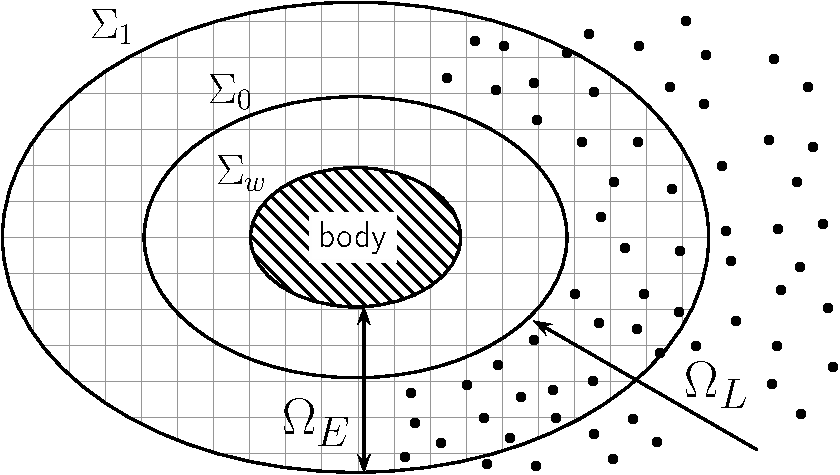
\includegraphics[width=0.6\linewidth]{figures/hybrid/domainDecomposition_typical_type2-crop.pdf}
			\caption{Standard domain decomposition using Schwartz iteration for coupling the two methods. Eulerian subdomain $\Omega_E$ (near the body), and Lagrangian subdomain $\Omega_L$ (away from the body). Figure is based on Guermond (2000) \cite{Guermond2000a}.}
			\label{fig:domainDecomposition}
		\end{figure}	
	
	Several studies have already been done: Cottet and Koumoutsakos (2000a)\cite{Cottet2000a}, Guermond and Lu (2000) \cite{Guermond2000a} simulated the advection dominated flows; Ould-Salhi et al. (2001) \cite{Ould-Salihi2001a} blended the finite difference and vortex method together; Winckelmans et al. (2005a) \cite{Winckelmans2005} investigated the trailing vorticies; Daeninck (2006) \cite{Daeninck2006} used a simplified coupling strategy, coupling Vortex Particle Method and Finite Diference Method; Stock (2010) \cite{Stock2010a} expanded Daeninck's strategy, coupling Vortex Particle Method and Finite Volume Method and modeled a 3D rotor.

	\section{Convectional Coupling Strategy}
	\label{sec:helvpm-ccs}
	
	When investigating the literature works, we see that not all domain decomposition methods are the same. The main difference between the methods is their coupling strategies. Most works employ the\textit{ Schwartz alternating method} to couple the vortex particle method and the grid solver. The Schwartz alternating method (or sometimes referred to as Schwartz iterative method), couples the vortex particle method and the grid solver by iteratively determining the boundary condition such that the stream functions in both domains, $\psi_L$ and $\psi_E$ in $\Omega_L$ and $\Omega_E$ respectively, match at the overlap region $\Omega_E-\Omega_L$, shown in Figure \ref{fig:domainDecomposition}. The summary of a single iteration of the Schwartz alternating method is as follows:
	
		\begin{itemize}
		\item Determine the Eulerian boundary condition, the stream function $\psi_{\Sigma_1}$ at the Eulerian boundary $\Sigma_1$, extracted from the Lagrangian stream function $\psi_L$ in the Lagrangian subdomain $\Omega_L$.
		\item Solve for the stream function $\psi_E$ in the Eulerian subdomain $\Omega_E$ with the new boundary condition $\Sigma_1$.
		\item Determine the Lagrangian condition, the stream function $\psi_{\Sigma_0}$ at the Lagrangian boundary $\Sigma_0$, extracted from the Eulerian stream function $\psi_E$ in the Eulerian subdomain $\Omega_E$.
		\item Solve the stream function $\psi_L$ in the Lagrangian subdomain with the boundary conditions $\psi_{\Sigma_0}$ at the Lagrangian boundary $\Sigma_0$.
		\end{itemize}
	
	This procedure is iterated until the stream functions of both domains converge \cite{Ould-Salihi2001a}. Once the stream function is determined in both the domains, the velocity field can be obtained. Using the velocity field, we can then evolve the vorticity field in the Lagrangian subdomain.

	\section{Simplified Coupling Strategy}
	\label{sec:helvpm-scs}
	
	As we realized now, the downside to this procedure is that we have to solve the stream function in both $\Omega_E$ and $\Omega_L$ iteratively, until we converge to a solution. This makes the computation very expensive, especially when we are dealing with large numbers of vortex particles. Therefore, for this project, we are using the coupling technique that is based on the research work of Daeninck (2006) \cite{Daeninck2006} and Stock (2010) \cite{Stock2010a}. However, through the course of present work, we will see that we have to perform a modification to the scheme, to ensure that the total circulation of the Lagrangian domain is conserved at all times.	
	
%	\subsection{Coupling Eulerian and Lagrangian Methods}
	
	The simplified coupling strategy was first demonstrated in the doctoral thesis of Daeninck \cite{Daeninck2006}. Daeninck showed that it is possible to coupled the Lagrangian and the Eulerian method without the use of Schwartz iterative method. Daeninck proposed this approach from the following statements:
	
	\begin{itemize}
	\item The Lagrangian vortex method solves the full fluid domain $\Omega_L$ (see Figure \ref{fig:domainDecomposition_daenick}), but under-resolves the near-wall region $\Omega_E$ as it is less efficient at resolving the boundary layer of the flow.
	
	\item Eulerian method is used to resolve the near-wall region $\Omega_E$, efficiently capturing the boundary layer features and flow separation.
	
	\item The Lagrangian subdomain in the near-wall region $\Omega_L\cap\Omega_E$ is corrected using the more accurate Eulerian solutions to compensate the aforementioned under-resolution.
	
	\item The boundary conditions for the Eulerian method is directly obtained from the evolved solution of the Lagrangian method.
	\end{itemize}
	
	The grid solver therefore essentially acts as the correction for the under-resolved regions of the Lagrangian method. The Lagrangian vortex method in the full fluid domain focuses only on capturing and efficiently evolving the wake.
	
		\begin{figure}[!h]
			\centering
			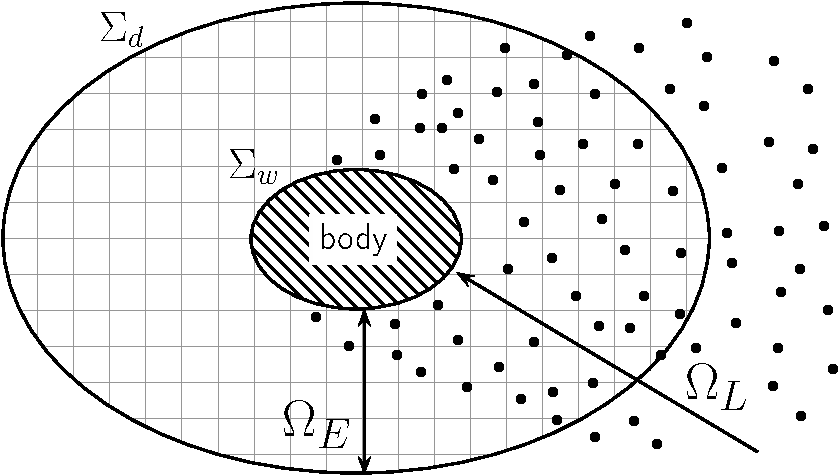
\includegraphics[width=0.6\linewidth]{figures/hybrid/domainDecomposition_daenick_type2-crop.pdf}
			\caption{Modified domain decomposition \underline{without} Schwartz alternating method. Lagrangian subdomain extends up to the surface of the body. Figure is based on Daeninck (2006) \cite{Daeninck2006}.}
			\label{fig:domainDecomposition_daenick}
		\end{figure}	
	
	Furthermore, Daeninck's simplified coupling strategy handles the Lagrangian boundary condition differently from the convectional domain decomposition method. In convectional method, the shedding of the vorticity from the wall is also defined in the Lagrangian method as well. However, in Daeninck's strategy, as the Lagrangian method is under-resolved at the boundary, it cannot be used to resolve the vorticity flux at the body. Instead, the Eulerian method is used to solve vorticity generation from the wall boundary, and acts as the vorticity generator for the Lagrangian method. 
	
	For this coupling strategy to be valid, there are some assumptions that we must satisfy:

	\begin{itemize}
	\item At $t_n$ before the evolution of both method to $t_{n+1}$, the Lagrangian solution matches Eulerian solution at the boundary of the near-wall region $\Sigma_d$ (see Figure \ref{fig:domainDecomposition_daenick}).
	\item Even though the Lagrangian subdomain is under-resolved in the near-wall region, it should still be able to provide accurate boundary conditions for the Eulerian method at the external boundary $\Sigma_d$.
	\item After the evolution to $t_{n+1}$, the deviation of the Lagrangian solution (due to lack of vorticity flux at Lagrangian boundary), should be minimal.
	\end{itemize}	
	
	Daeninck's the simplified coupling strategy focused on the vorticity-velocity formulation for the Eulerian domain. However, he briefly showed that it is also possible to couple the Eulerian method with the velocity-pressure formulation. The advantage of using the velocity-pressure formulation is that it will be easier to extend to a 3D problem, unlike the vorticity-velocity formulation for the Eulerian method.
	
	\subsection{Coupling Algorithm}	
	
	The coupling of the solvers was described in one global time stepping algorithm. As the Eulerian methods suffers from a larger stability constraint on the time step, and the Lagrangian time marching is computationally more expensive, a  different time discretization for both methods was employed. The Lagrangian method and the Eulerian method had the time steps $\Delta t_L$ and $\Delta t_E=\Delta t_L/k_E$, respectively, where $k_E$ is the number of Eulerian sub-steps.
	
	Assuming that we known the solutions of both solver at $t_n$, the algorithm for the coupled time marching from $t_n$ to $t_n+\Delta t_L$ for Eulerian method (with velocity-pressure formulation) and the Lagrangian method is summarized as follows:
	
	\begin{enumerate}
	\item At $t_n$, \textbf{correct the Lagrangian solution} in the near-wall region $\Omega_L\cap\Omega_E$ from the Eulerian field, Figure \ref{fig:domainDecomposition_daenick}. The vorticity in $\Omega_E$ is determined by taking the curl of the velocity field of the Eulerian method. The vortex particles strengths are determined by interpolating the vorticity from the Eulerian grid.
	
	\item \textbf{Advance the Lagrangian method} from $t_n$ to $t_{n}+\Delta t_L$, with the corrected Lagrangian solution. Before the evolution, there exists a slip velocity at the solid wall $\Sigma_w$. Therefore, the vortex method needs to enforce the \textit{no-slip} boundary condition at the wall by computing the vortex sheet $\gamma$ that cancels this slip velocity. At the end of the evolution, classic vortex methods diffuse the computed vortex sheet to the particles but in Daeninck's work, it is handled by the Eulerian method.
	
	\item\textbf{ Determine the Eulerian boundary conditions} for the velocity field $\mathbf{u}$ at $t_{n}+\Delta t_L$ from the Lagrangian solution at $t_{n} + \Delta t_L$. The Eulerian method requires the Dirichlet velocity boundary condition at $\Sigma_d$ (the Eulerian Dirichlet velocity boundary). The velocity boundary condition at the wall boundary $\Sigma_w$ for a velocity-pressure formulation is simply the zero slip velocity. 
	
	\item \textbf{Advance the Eulerian method} from $t_n$ to $t_n + \Delta t_L$ using $k_E$ Eulerian substeps. The boundary conditions on $\mathbf{u}$ at each substep is obtained by linear interpolation of the boundary condition at $t_n$ and $t_{n} + \Delta t_L$.
	\end{enumerate}	
	
	To enhance the coupling of the Eulerian and the Lagrangian method, Daeninck further modified the Eulerian solution in the most external region of the Eulerian subdomain $\Omega_E$ from interpolation the Lagrangian solution, and observed that it provided better results. Figure \ref{fig:daeninckInterpolation} the modified adjustments regions used by Daeninck in his work.
	
	\begin{figure}[!t]
		\centering
		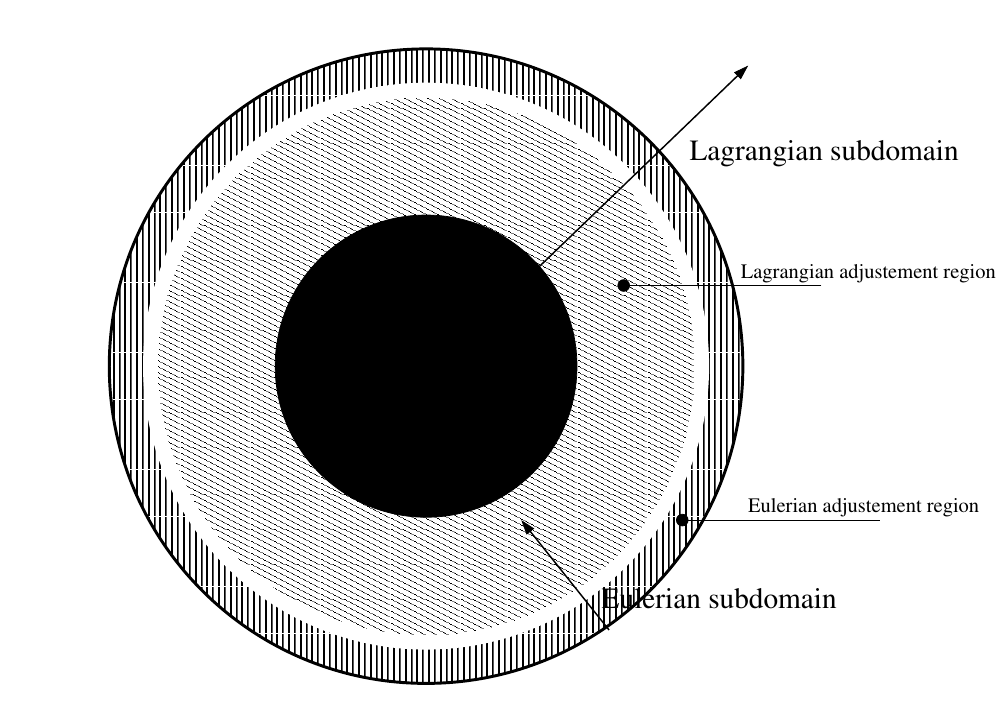
\includegraphics[width=0.6\linewidth]{figures/hybrid/daeninckInterpolationRegions.png}
		\caption{The domain decomposition and interpolation regions used by Daeninck \cite{Daeninck2006}. The Eulerian domain is also modified to enchace the coupling of the methods.}
		\label{fig:daeninckInterpolation}
	\end{figure}		
	
	\subsection{Lagrangian Correction Step}
	
	The coupling strategy demonstrated by Daeninck \cite{Daeninck2006}, was studied and was further extended by Stock \cite{Stock2010a}. Stock's work focused on the overlap region $\Omega_E\cap\Omega_L$ (Figure \ref{fig:domainDecomposition_daenick}) and correction of the Lagrangian solution. Following observations was determined by the work:
	
	\begin{itemize}
	\item Eulerian solution is only assumed to be correct from the body surface $\Sigma_w$ to somewhat inside of the outer Eulerian domain $\Sigma_d$. Therefore, the transfer of the Eulerian solution to the Lagrangian method should take in account of the potential inaccuracy of the Eulerian solution at the outer boundary.
	
	\item The very strong gradient in vorticity (vortex sheet) cannot be efficiently and accurately transfered to the Lagrangian method. This is especially problematic at high Reynolds number flows, and interpolating this vorticity from Eulerian method to Lagrangian method results in numerical problems. Therefore, to avoid the noise in the interpolation, the correction step has to ignore the region very near to the wall.
	\end{itemize}
	
	The resulting Lagrangian correction domain, or the interpolation domain $\Omega_I$, using Stock's coupling approach is shown in Figure \ref{fig:interpolationDomainDefinition}. The interpolation domain $\Omega_I$ is defined with an offset from the Eulerian domain boundaries $\Omega_E: \partial\Omega_E=\Sigma_w \cup \Sigma_d$, Figure \ref{fig:interpolationDomainExpanded}, such that regions of the Eulerian domain that introduces issues with coupling are ignored. The outer boundary of the interpolation domain $\Sigma_i$ is defined with an offset $d_{bdry}$ from the Eulerian Dirichlet velocity boundary $\Sigma_d$ such that potential inaccuracy of the Eulerian solution is ignored, shown in Figure \ref{fig:interpolationDomainCloseup}. Similarly, the inner boundary of the interpolation domain $\Sigma_o$ is defined with an offset $d_{surf}$ from the Eulerian wall boundary $\Sigma_w$ such that the very strong vorticity is ignored. The offsets $d_{surf}$ and $d_{bdry}$  where defined in the order of the Lagrangian vortex particle size.
	
	\begin{figure}[!t]
        \centering
        \begin{subfigure}[b]{0.45\textwidth}
                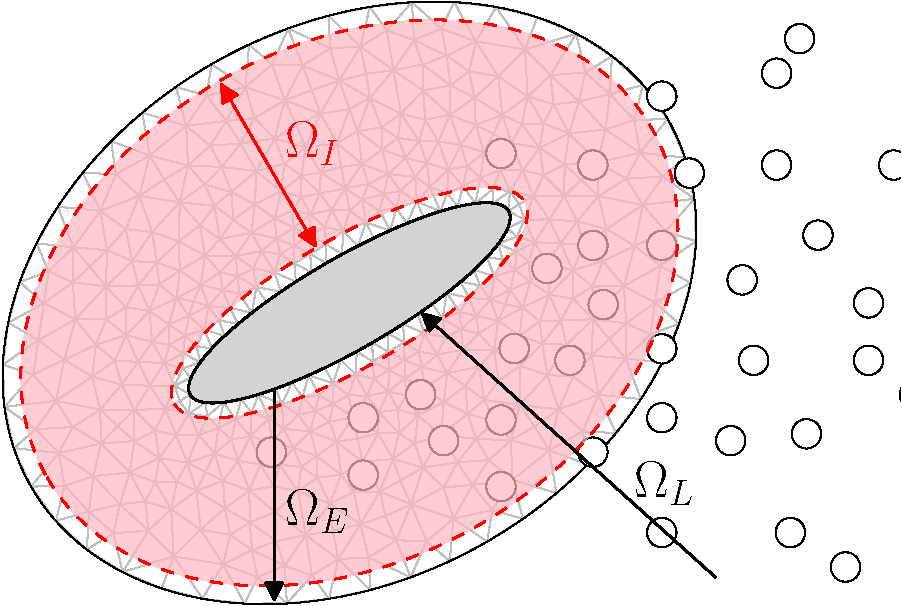
\includegraphics[width=\textwidth]{figures/hybrid/interpolationDomain/interpolationDomainExpanded-crop.pdf}
                \caption{Definition of the Domains}
                \label{fig:interpolationDomainExpanded}
        \end{subfigure}%
        \qquad %add desired spacing between images, e. g. ~, \quad, \qquad etc.
          %(or a blank line to force the subfigure onto a new line)
        \begin{subfigure}[b]{0.45\textwidth}
                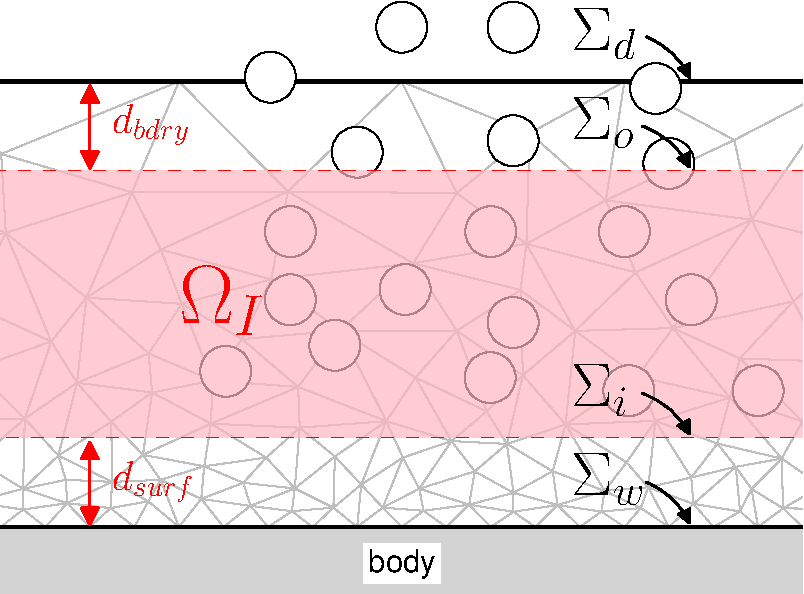
\includegraphics[width=\textwidth]{figures/hybrid/interpolationDomain/interpolationDomainCloseup-crop.pdf}
                \caption{Definition of the boundaries}
                \label{fig:interpolationDomainCloseup}
        \end{subfigure}
        \caption{Definition of the interpolation domain $\Omega_{int}$ for correcting the Lagrangian solution, with boundaries $\Omega_I: \partial\Omega_I=\Sigma_{i}\cup\Sigma_{o}$.}
        \label{fig:interpolationDomainDefinition}
	\end{figure}		

	The resulting Lagrangian correction step employed by Stock is summarized as follows:
	
	\begin{enumerate}
	\item Interpolate the vorticity of the Eulerian method from a non-uniformly structured (or an unstructured grid) onto a temporary uniformly structured Cartesian grid covering the entire Eulerian domain $\Omega_E$. This is done to performed an easier correction of the Lagrangian solution with the Eulerian solution. The interpolation ignores the very strong vorticity present in the boundary layer that could cause numerical problem.
	\item Determine all the particles within the interpolation domain $\Omega_I$ that is to be corrected.
	\item Correct or reset the strengths of the particles using the local particle area and the vorticity interpolated from the temporary structured Cartesian grid.
	\end{enumerate}
	
	Using this approach, Stock demonstrated the feasibility of simulating a 3D compressible flow problem around a sphere at $Re=100$, a finite airfoil at $Re=\num{1.5e6}$, and 4-Bladed advancing rotor at $Re=865,500$.
	
	\section{Evolution of the Hybrid Method}

	In the present work, we will therefore employ Daeninck's simplified coupling strategy with the detailed Lagrangian correction approach of the Stock. The evolution of the hybrid method is classified into four parts and is as follows:

		\begin{enumerate}
		\item \textbf{Correct Lagrangian:} Use the solution of the Eulerian subdomain $\Omega_E$, to correct the solution of the Lagrangian subdomain $\Omega_L$, using the strategy of Stock. Chapter \ref{ch:coupling} provides a detailed investigation on the implementation of Stock's Lagrangian correction strategy. However, during the implementation, we saw that conservation of total circulation in the Lagrangian method is paramount for an accurate correction.
		
		\item \textbf{Evolve Lagrangian:} With the modified solution, evolve the Lagrangian solution from time step $t_n$ to $t_{n}+\Delta t_L$. Chapter \ref{ch:lagrangian} provides the detailed investigation on the theory and the algorithm of the Lagrangian method used for the present work.
		
		\item \textbf{Determine Eulerian boundary conditions:} Use the Lagrangian solution of time $t_{n}+\Delta t_L$ to determine the boundary conditions of the Eulerian subdomain at $t_{n}+\Delta t_L$.
		
		\item \textbf{Evolve Eulerian:} With the boundary condition, evolve the Eulerian solution from $t_n$ to $t_{n}+\Delta t_L$ using $k_E$ Eulerian substeps. Chapter \ref{ch:eulerian} provides the detailed investigation on the theory and the algorithm of the Eulerian method used for the present work.
		\end{enumerate}
	
	Figure \ref{fig:flowchart_simpleCoupling} shows the flowchart of the evolution of the hybrid method. To ensure that the coupling of the hybrid method performs as explained in theory, we required a verification and validation test on the functionality of each segregate methods.
	
	
	\begin{figure}[!t]
		\centering
		\begin{tikzpicture}
			[node distance=.8cm, start chain=going below,]
			\node[punktchain, join] (correct) {Correct the \\Lagrangian subdomain};
		    \node[punktchain, join] (evolveL) {Evolve the Lagrangian solution};
		    \node[punktchain, join] (bcE)     {Determine the \\Eulerian boundary conditions};
		    \node[punktchain, join] (evolveE) {Evolve the Eulerian solution};
		\end{tikzpicture}
		\caption{Flowchart of the simple coupling strategy. The flowchart shows the procedure to evolve both methods from $t_n$ to $t_{n+1}$.}
		\label{fig:flowchart_simpleCoupling}
	\end{figure}




% Summarize daenincks approach:
	% Methodology, algorithm
	% Domain decomposition
% Summarize stock's approach:
	% Methodology, algorithms
	% Resulted domain decomposition.


%%%%%%%%%%%%%%%%%%%%%%%%%%%%%%%%%%%%%%%%%%%%%%%%%%%%%%%%%%%%%%%%%%%%%%%%%%%%%%%%%%%%%%%%%%%%%%%%%%%%%%%%%%%%%%%%%%%%%%%%%%%%%%%%%%



